\documentclass[twocolumn]{article}
\usepackage[margin=0.75in]{geometry}
\usepackage{graphicx}
\setkeys{Gin}{width=\columnwidth, keepaspectratio}
\usepackage{amsmath, amssymb}
\usepackage{hyperref}
\usepackage{multicol}
\usepackage{url}
\usepackage{subcaption}
\def\UrlBreaks{\do\/\do-} %% NEED THIS TO WRAP AROUND LONG URLS

\title{Final Report: NLP-Driven Financial Sentiment Analysis and Risk Scoring}
\author{NDR Team \#4: Brian Adams, Hilung Huang, Luis Tupac\\NED Davis Research – Practicum, GT - Spring 2025}
\date{\today}

\begin{document}
\maketitle

\begin{abstract}
This report presents a comprehensive study on predicting market volatility using Natural Language Processing (NLP) techniques applied to financial headlines and SEC filings. Conducted in collaboration with Ned Davis Research (NDR), our objective was to develop robust "Risk Scores" for the S\&P 500 index and its constituents that anticipate significant stock price movements. We investigated multiple modeling strategies, including token-level sentiment scoring, VIX-based volatility modeling, and topic modeling using BERTopic. Our findings highlight the predictive power of combining token-level features with sentiment and high-risk language metrics, particularly when sufficient article volume is available. Notably, a single engineered token-focused risk feature demonstrated superior performance and stability over more complex multi-feature models. We conclude by proposing future enhancements such as segmentation-based modeling, ensemble learning, and reinforcement learning to further improve accuracy and scalability.
\end{abstract}

\section{Introduction}
\subsection{Project Aim}
This project, conducted in collaboration with \textbf{Ned Davis Research (NDR)}, explores the predictive power of aggregated sentiment indicators derived from financial data and SEC filings to identify potential market inflection points. By leveraging \textbf{Natural Language Processing (NLP)} and financial analytics, our objective is to create a comprehensive "Risk Score" for the S\&P 500 index and its historical constituents.

\subsection{Background and Motivation}
Investment sentiment plays a crucial role in market trends. News articles and SEC filings impact market movements by emphasizing risk-laden keywords such as ``bankrupt'' and ``lawsuit.'' The goal is to quantify the relationship between sentiment trends and financial health, thereby better predicting market volatility.

\subsection{Project Objectives}
\begin{itemize}
    \item \textbf{Data Collection:} Collect data from the sponsor.
    \item \textbf{High-Risk Dictionary:} Aggregate high-risk words from news headlines and SEC filings (with emphasis on 10-K reports, particularly Items 1 and 1A).
    \item \textbf{Risk Score Development:} Create a Risk Score to help investors anticipate market drops.
\end{itemize}

\section{Literature Review}
%%%%%%%%%%%%%%%%%%%%%%%%%%%%%%%%%%%%%%%%%%%%%%%%%%%%%%%%%%%%%%%%%%%%%%%%%%%%%%
%%%%%%%%%%%%%%%%%%%%%%%%%% Luis Literature reviews %%%%%%%%%%%%%%%%%%%%%%%%%%
%%%%%%%%%%%%%%%%%%%%%%%%%%%%%%%%%%%%%%%%%%%%%%%%%%%%%%%%%%%%%%%%%%%%%%%%%%%%%%
\subsection{FinBERT: Financial Sentiment Analysis with BERT}
FinBERT is a language model tailored for financial text analysis, built by fine-tuning BERT on a financial corpus~\cite{genc2020finbert}. It leverages transformers to enable bi-directional processing of financial texts. The model is trained to understand how to talk like a trader by using a financial corpus and labeled data for financial sentiment classification. The model outperformed other models like LSTM, LSTM with ELMo, ULMFit, and BERT, with a 97\% accuracy on the subset. While the model improves sentiment prediction for complex financial texts, it is not able to capture all forms of "trader speak," which is a form of manipulating neutral or negative statements to sound better than normal. \\
\textbf{Example Statement:} \\ 
\textit{This implementation is very important to the operator, since it is about to launch its Fixed to Mobile convergence service in Brazil}
\begin{itemize}
    \item \textbf{True value}: Neutral
    \item \textbf{Predicted}: Positive
\end{itemize}

Even with its limitations, it represents a significant advancement over general-purpose sentiment models in financial applications. This paper inspired us to combine FinBERT sentiment and embeddings into our models in an effort to extract as much information as possible from the provided articles.

\subsection{Automatic Text Summarization Using Gensim Word2Vec and K-Means}
Haider et al.~\cite{9230670} proposed an interesting method for automatic text summarization by combining Word2Vec embeddings from the Gensim library with K-Means clustering. Their approach transforms sentences into vector representations and groups semantically similar sentences to extract meaningful summaries. 
The authors used clustering on the embedded sentences to identify representative sentences from each cluster to summarize the input document. This method works well for single-document extractive summarization and highlights the potential of word embeddings and clustering for structuring unlabeled text. 

Their work inspired our decision to use Word2Vec for financial news embeddings, though we adapted the clustering strategy to DBSCAN and HDBSCAN for better noise handling and density based grouping in our financial articles.

%%%%%%%%%%%%%%%%%%%%%%%%%%%%%%%%%%%%%%%%%%%%%%%%%%%%%%%%%%%%%%%%%%%%%%%%%%%%%%
%%%%%%%%%%%%%%%%%%%%%%%%%% Literature reviews %%%%%%%%%%%%%%%%%%%%%%%%%%
%%%%%%%%%%%%%%%%%%%%%%%%%%%%%%%%%%%%%%%%%%%%%%%%%%%%%%%%%%%%%%%%%%%%%%%%%%%%%%



\subsection{Investor Sentiment and Market Trends}
Tetlock’s research shows that negative sentiment in news articles (e.g., from the Wall Street Journal) can predict lower future stock returns and heightened market volatility. This insight is reflected in our incorporation of sentiment polarity in the Risk Score computation.

\subsection{Event-Based Financial Modeling}
Research by Hu and colleagues demonstrates that detecting significant financial events through NLP improves stock return predictions. This approach motivates our keyword-based method for tracking price swings by identifying events such as earnings reports, legal issues, and downgrades.

\subsection{Bollinger Bands}
Developed by John Bollinger, Bollinger Bands® are volatility bands placed above and below a moving average. Volatility is based on the standard deviation, which changes as volatility increases and decreases. Bollinger Bands consist of three lines: a simple moving average (SMA) line, an up-per band, and a lower band. The SMA line is the average price over a specified period of time, in our case 5 days for strategy learner and 14 days for manual learner. The upper band is two standard deviations above the SMA line, and the lower band is two standard deviations below the SMA line.~\cite{chartschool_bollinger}

\subsection{Relative Strength Index (RSI)}
Developed by J. Welles Wilder, the Relative Strength Index (RSI) is a momentum oscillator that measures the speed and change of price movements. RSI oscillates between zero and 100. RSI is considered overbought when above 70 and oversold when below 30.~\cite{chartschool_rsi}

\subsection{Stochastic Oscillator}
Developed by George C. Lane in the late 1950s, the Stochastic Oscillator is a mo-mentum indicator that shows the location of the close relative to the high-low range over a set number of periods.~\cite{chartschool_stochastic}


\section{Exploratory Data Analysis (EDA)}
We created a database following the Medallion architecture pattern which consists of Bronze, Silver, and Gold data layers. All of the raw data landed as is into the bronze layer, where it was then curated into the silver layer, and finally had aggregations and joins performed to it that allowed us to efficiently use it for our downstream experimentation.

The Medallion architecture consists of three distinct data layers:

\begin{itemize}
    \item \textbf{Bronze:} Raw, unprocessed data ingested from source systems.
    \item \textbf{Silver:} Cleaned, structured, and joined data that is ready for analytics.
    \item \textbf{Gold:} Aggregated, curated datasets optimized for modeling and experimentation.
\end{itemize}
\begin{figure}[h!]
    \centering
    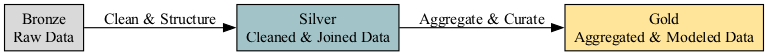
\includegraphics[width=0.45\textwidth]{medallion_architecture.png}
    \caption{Medallion Architecture Diagram.}
    \label{fig:modeling-evolution}
\end{figure}

We followed this pattern to structure the data efficiently and make it analyzable data. This database consists of 3 schemas:
\begin{enumerate}
    \item Headline Schema
    \item SP500 Schema
    \item Test Schema
\end{enumerate}


\subsection{Headline Schema}
\begin{figure}[h!]
    \centering
    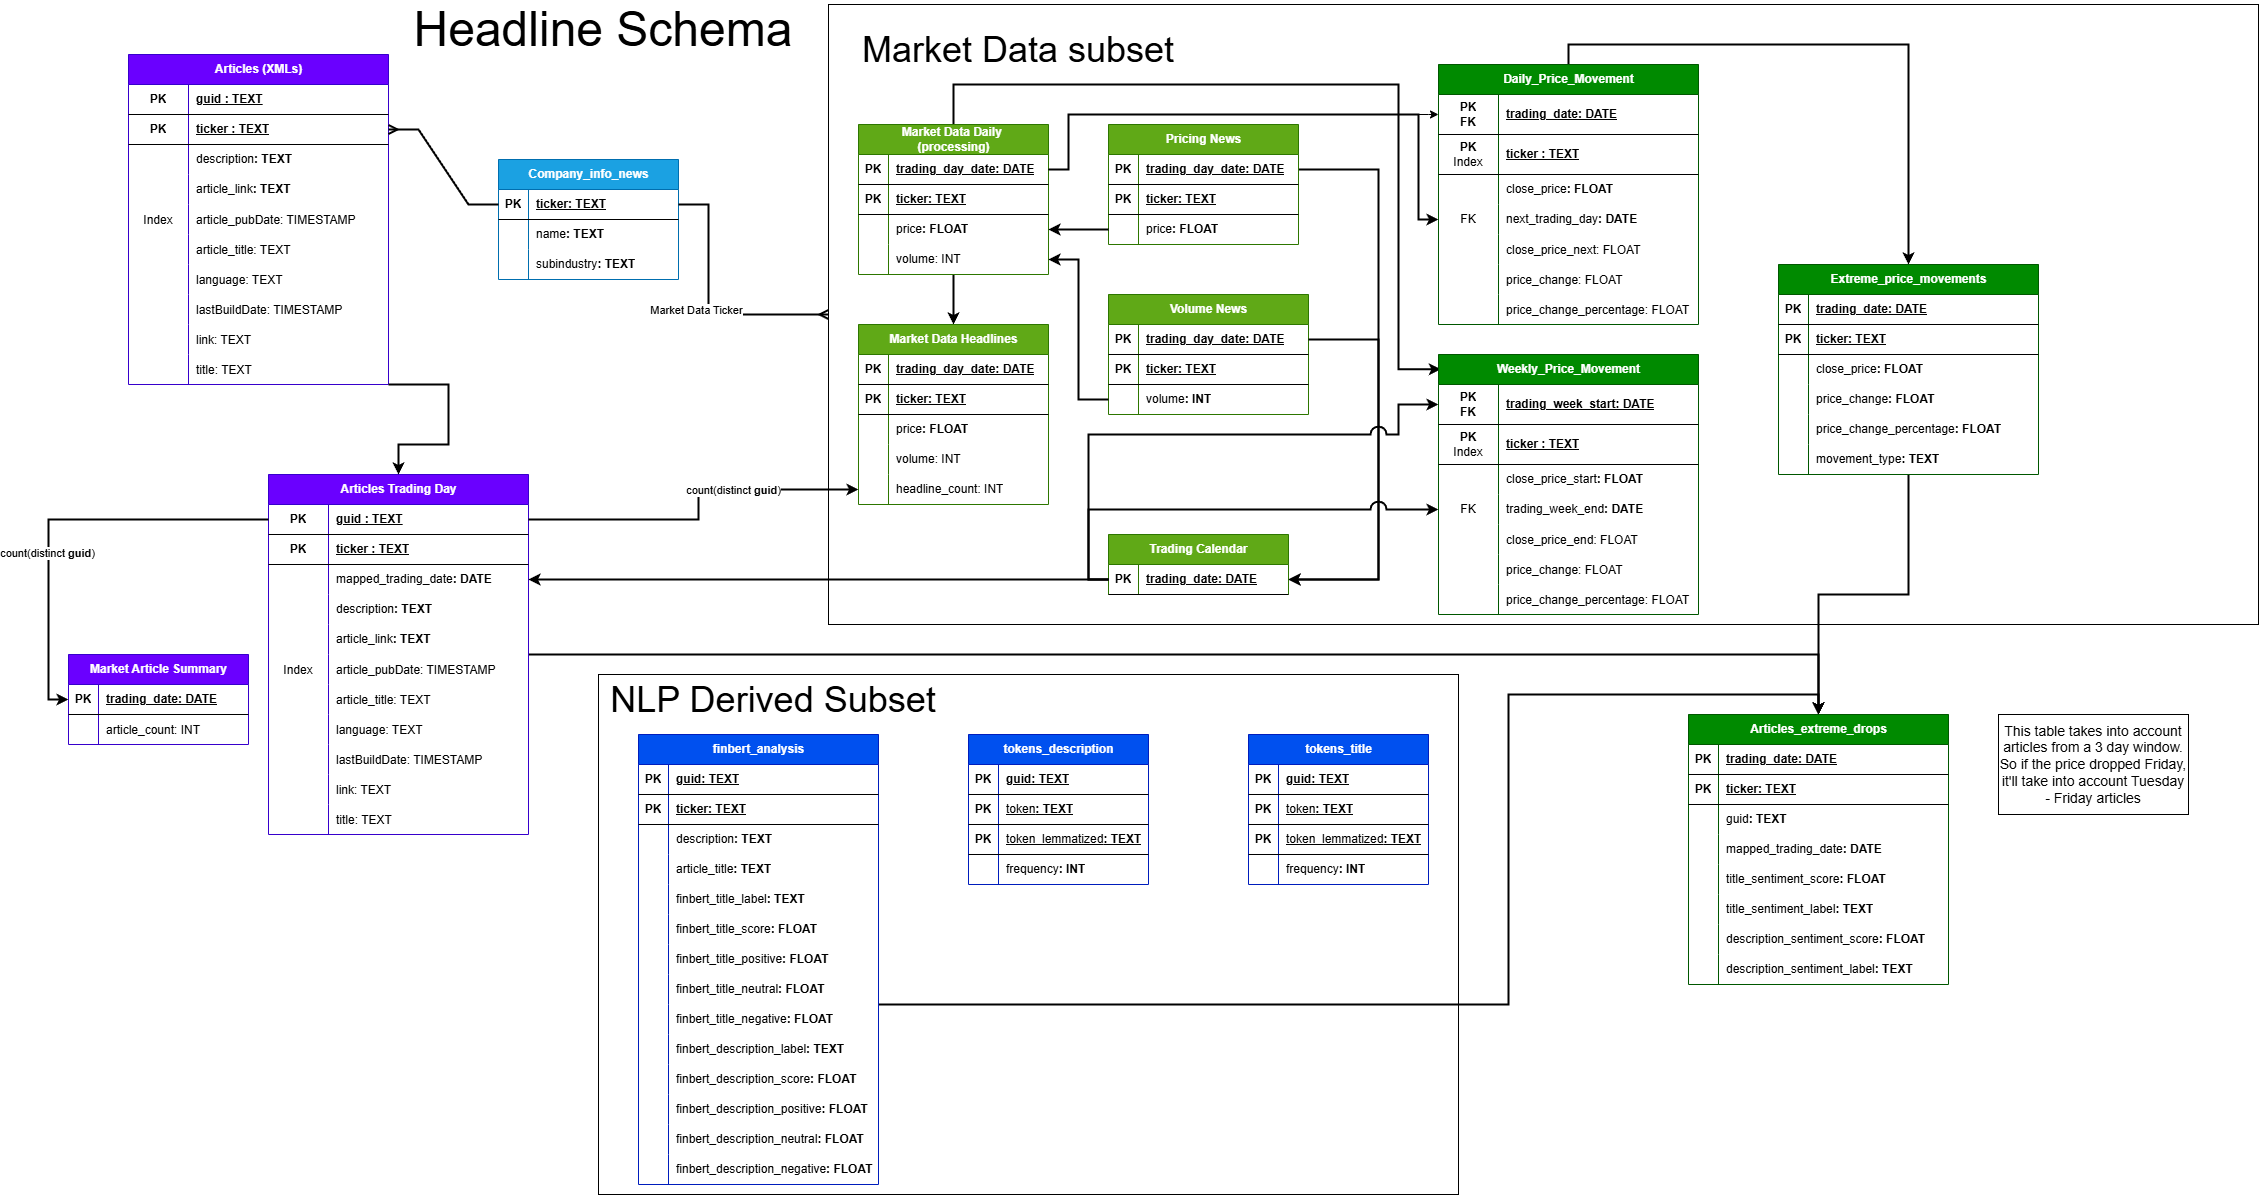
\includegraphics[width=0.5\textwidth]{headlines_schema.png}
    \caption{Headline Schema.}
    \label{fig:headline-schema}
\end{figure}

This schema held our most important data and housed key data and transformations such as:
\begin{itemize}
    \item Ticker article data
    \begin{itemize}
        \item These were raw XML files which we had to parse, sanitize, and link to tickers. 
        \item Some challenges from this dataset included parsing the special characters, handling encoding errors, and aligning articles published after market close to the next available trading day. Aligning the articles was a key part of our analysis since it gave us the ability to see the impact an article had on price.
    \end{itemize}
    \item Financial market data 
    \begin{itemize}
        \item This consisted of daily price and volume information for all the tickers provided to us. This was specially tricky since the data was stored in a matrix format (tickers as columns, dates as rows) which is visually pleasing when viewing the data, but not helpful when performing aggregations. We transformed this data into a long format structure, allowing us to perform critical operations and allowing us to infer additional data easier, like inferring the market calendar for the data we were given without relying on external datasets.
    \end{itemize}
    \item FinBERT sentiments
    \begin{itemize}
        \item We built a custom FinBERT pipeline to extract \textbf{\textit{all}} sentiment scores and labels (positive, neutral, negative) instead of relying on the default return of top label and score from default pipeline.
        \item This custom pipeline consisted of:
        \begin{enumerate}
            \item Creating a distributed network with Dask (since we did not have access to GPUs).
            \item Run FinBERT in a custom inference loop.
            \item Extract logits and using Softmax to convert them into probability distributions. 
        \end{enumerate}
        \item This custom loop enriched our downstream modeling by providing us with additional information on article sentiment we didn't have before.
    \end{itemize}
    \item Extreme price movements
    \begin{itemize}
        \item We tracked all price movements and flagged the tickers that had a $\pm5\%$ price change from previous close. This system captured the data from the past three trading days to identify factors for this kind of movement. 
    \end{itemize}
\end{itemize}

This schema combined with the seamless integration we received from DuckDB allowed us to quickly prototype by minimizing the time spent on data cleaning and data integration used in our notebooks.

\subsection{SP500 Schema}
\begin{figure}[h!]
    \centering
    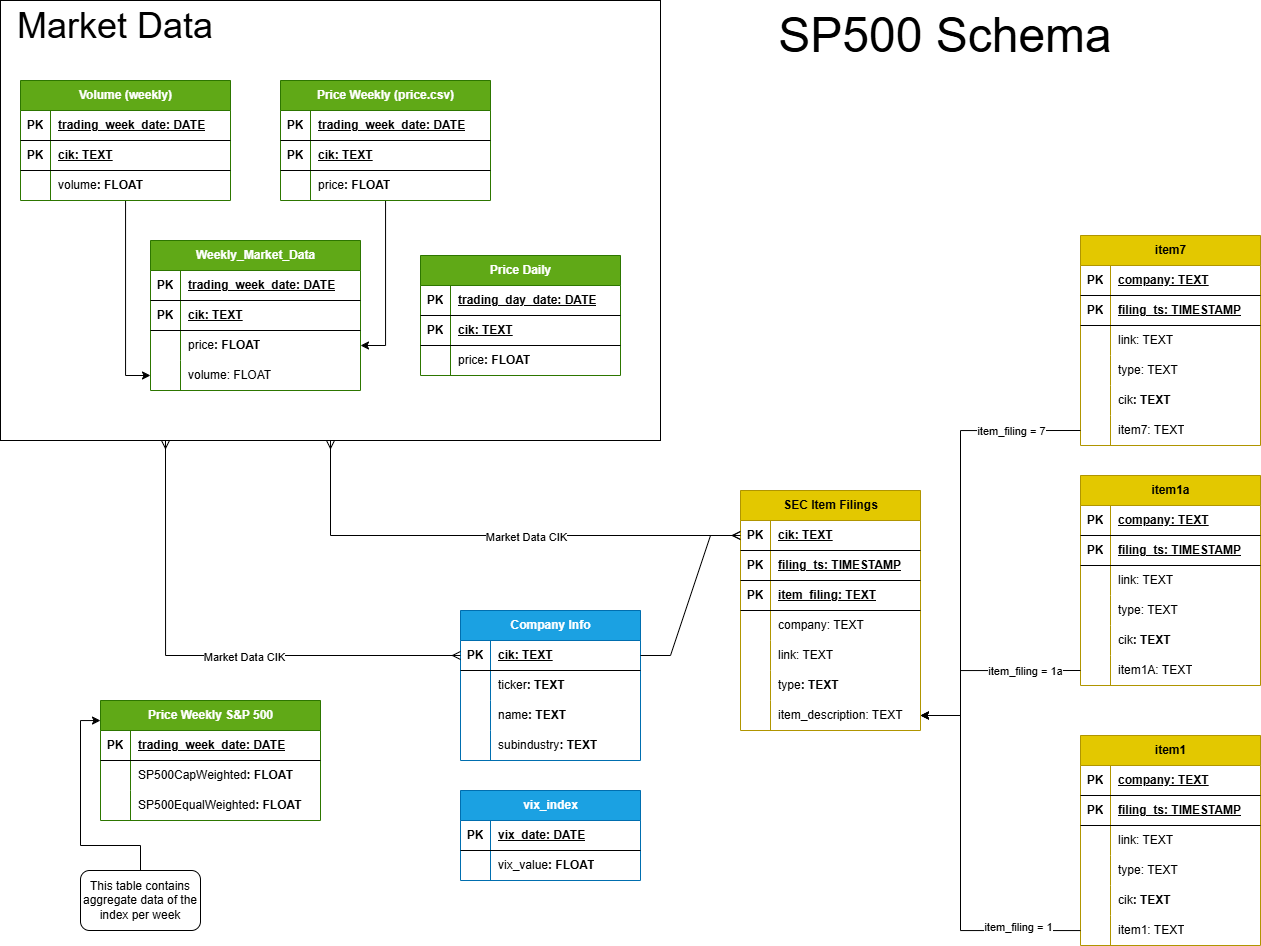
\includegraphics[width=0.5\textwidth]{sp500_schema.png}
    \caption{SP500 Schema.}
    \label{fig:headline-schema}
\end{figure}

This schema consisted of financial data for the S\&P500 companies and SEC item filings. This schema was not the core focus of the project, it mainly served as a valuable extension to our Headline data. 

The main aggregations are similar to the Headline aggregation with us:
\begin{itemize}
    \item Flattening Volume and Price data.
    \item Flattening SEC filings.
    \item Performing FinBERT sentiment analysis to the SEC filings.
\end{itemize}

A key feature we used from this schema was the VIX index, which became an important input to many of our models.

\subsection{Test Schema}
\begin{figure}[h!]
    \centering
    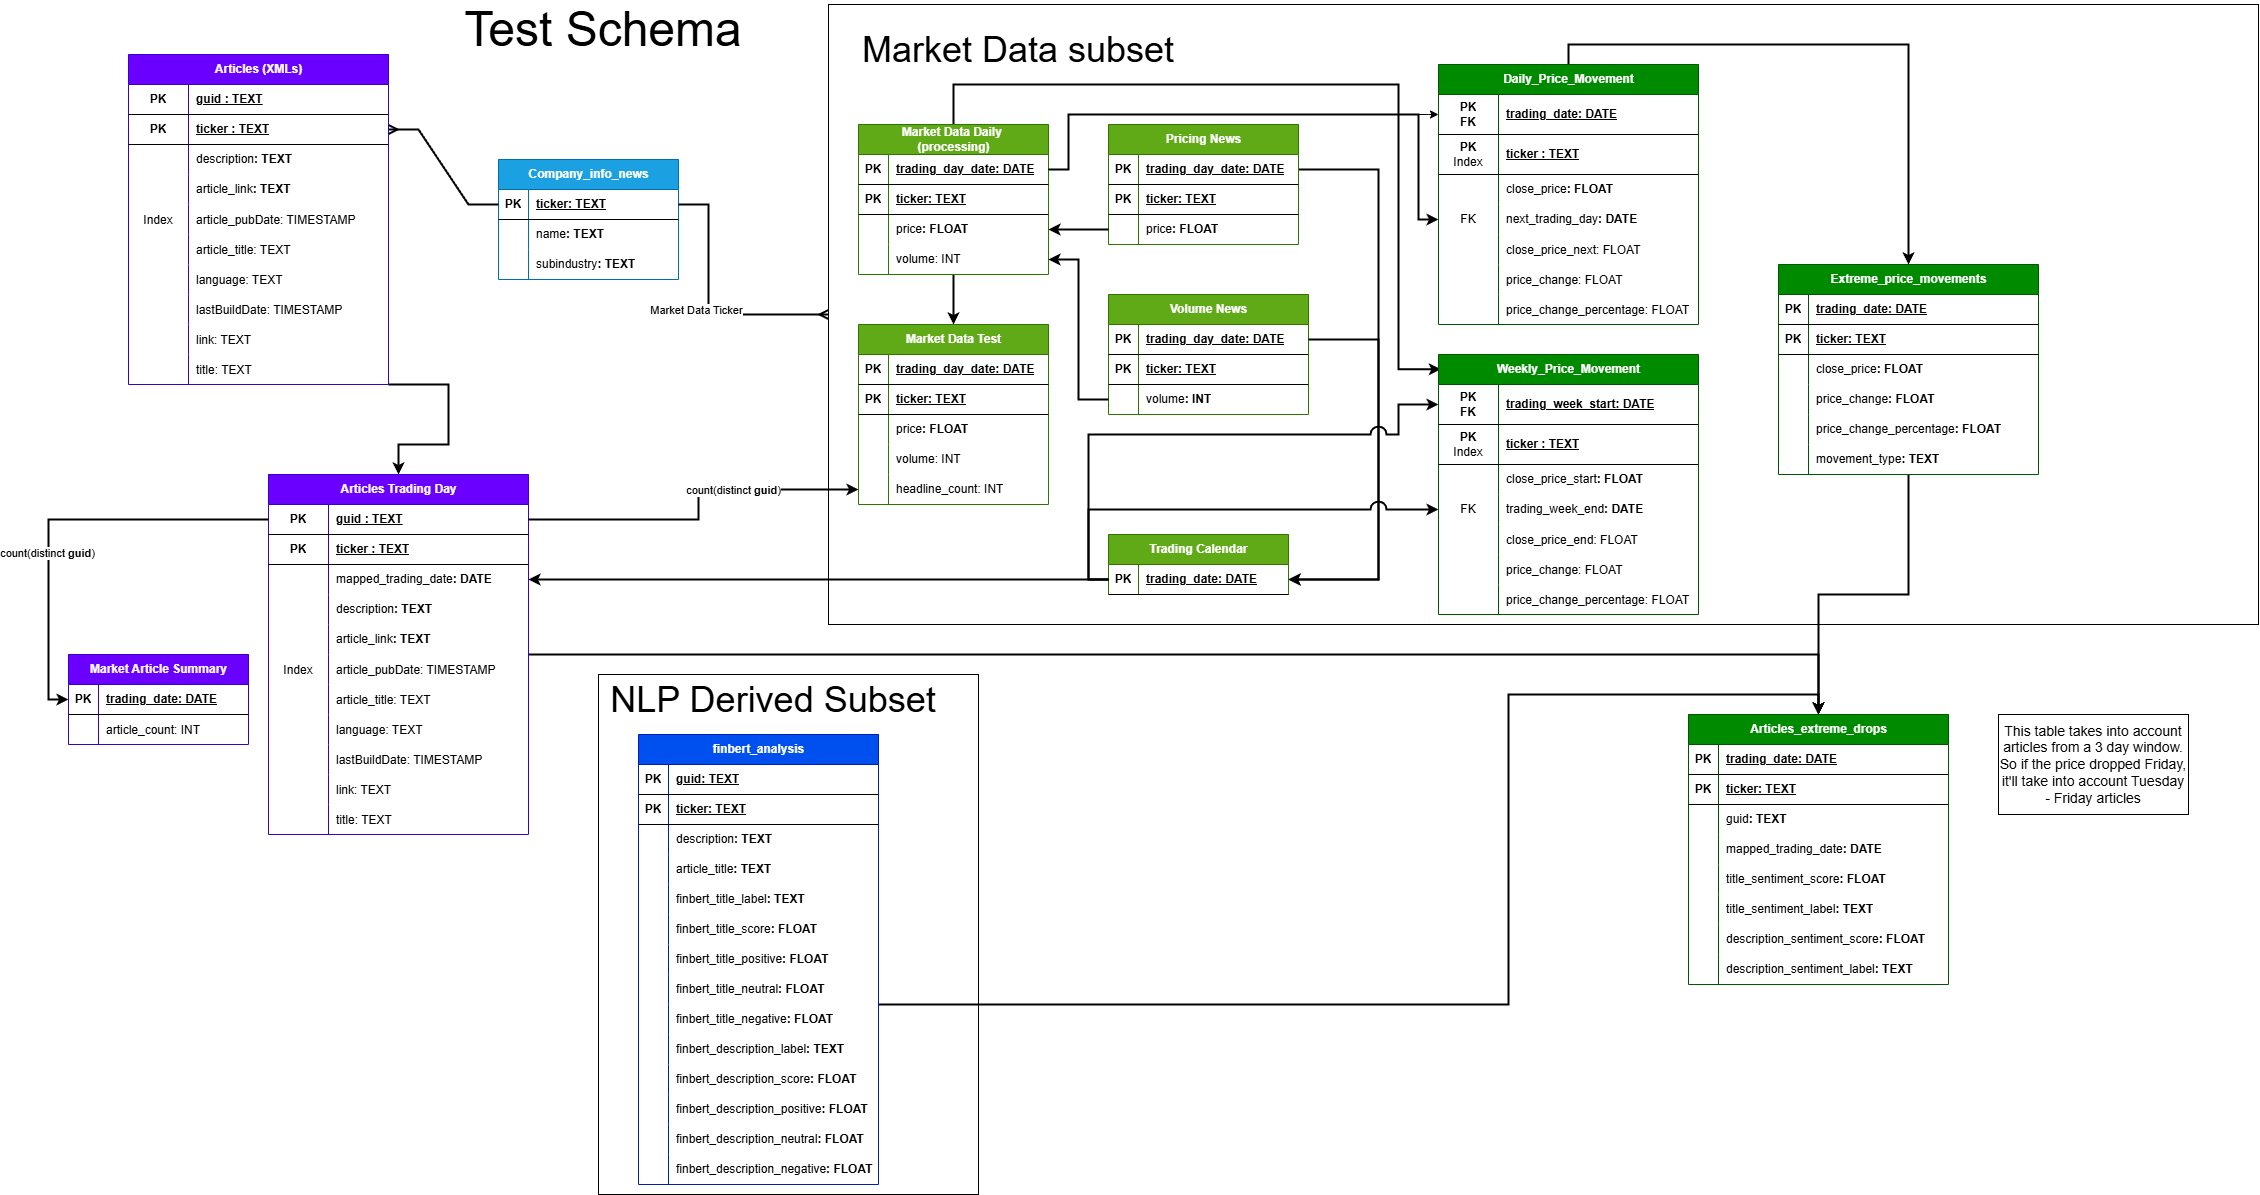
\includegraphics[width=0.5\textwidth]{test_schema.png}
    \caption{Test Schema.}
    \label{fig:headline-schema}
\end{figure}

The Test schema was modeled after the Headline schema and was used to hold newly provided data from our sponsor. We ran this data through the same curation pipelines as the Headline schema. This provided us with identical table structures, with a few small adjustments like removing unused tables and renaming tables.

Although this schema may look simple, having the test data available in table format made a huge difference. By loading it directly into DuckDB we were able to use its integration with Python to rapidly iterate on our models and evaluate performance on this new data with minimal adjustments to our existing training pipelines.

\section{Model Survey and Methodology}

Our project has evolved significantly through extensive experimentation with diverse modeling strategies. We surveyed several approaches, ranging from traditional predictive methods to sophisticated NLP-driven techniques, aiming to derive insightful risk metrics that anticipate stock price volatility. This section introduces these modeling approaches, highlighting their theoretical foundations and practical implementation considerations, leading logically into our detailed experiments and results.

\begin{figure}[h!]
    \centering
    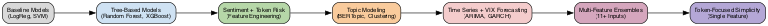
\includegraphics[width=0.45\textwidth]{modeling_progression_diagram.png}
    \caption{Evolution of Modeling Complexity.}
    \label{fig:modeling-evolution}
\end{figure}

\subsection{Baseline and Initial Modeling Approaches}
We began our analysis with standard statistical and machine learning models to benchmark performance:
\begin{itemize}
    \item \textbf{Logistic Regression:} Employed initially for binary classification of price movements.
    \item \textbf{Support Vector Machines (SVM):} Selected for effectiveness in handling text-based feature spaces.
    \item \textbf{Random Forest and XGBoost:} Tested for capturing complex, nonlinear interactions among features.
\end{itemize}

These models established performance baselines and guided subsequent methodological refinements.

\subsection{Advanced Sentiment and Token-Level Analytics}
We significantly enhanced our modeling by incorporating sentiment analysis and detailed token-level analytics, leveraging FinBERT's financial-specific transformer model:
\begin{itemize}
    \item \textbf{Sentiment Analysis Integration (FinBERT):} Extracted nuanced sentiment scores beyond simple positive-negative labels to gain deeper predictive signals from news headlines and SEC filings.
    \item \textbf{Token-Level Risk Scores:} Developed features such as sentiment volatility, high-risk word variability, and token-score metrics. Experimentation identified a comprehensive “Token-Focused” risk metric that notably improved correlation with market volatility.
    \item \textbf{Weighted Risk Score Experiments:} Evaluated multiple weighting schemes—equal, sentiment-focused, high-risk-focused, and token-focused—to maximize predictive accuracy.
\end{itemize}

\subsection{NLP: Named Entity Recognition (NER)}
We also incorporate NER from spaCy library to increase our prediction accuracy. We removed all NER categories to achieve: 
\begin{itemize}
    \item \textbf{Reducing Noise in Text Classification:} Named entities (like names, dates, or locations) may add irrelevant variation and reduce our model performance and accuracy. Removing them can help the model focus on core linguistic or semantic patterns.
    \item \textbf{Improving Generalization in Models:} Names and specific references can overfit models to particular examples. Removing or replacing entities (e.g., with placeholders like PERSON or ORG) makes the model more robust.
    \item \textbf{Enhancing Keyword or Topic Extraction:} Entities like names and dates can crowd out meaningful keywords. For instance, we use weighted average in our token score/risk score. In this case, "Recession" should have a high negative value or weighted average. However, by allowing less meaningful words such as Saturday, three... We can actually reduce the score of "Recession".
\end{itemize}

\subsection{Time-Series Modeling with VIX}
Recognizing the importance of broader market sentiment captured by the VIX volatility index, we:
\begin{itemize}
    \item Conducted exploratory correlations between VIX and future price movements.
    \item Built predictive models (ARIMA, ARMA-GARCH) to forecast VIX values, employing them as additional features for predicting stock price volatility.
\end{itemize}

These experiments validated our hypothesis regarding the delayed market impact of volatility signals, particularly under moderate VIX conditions.

\subsection{Topic Modeling Approaches (BERTopic)}
To uncover latent thematic drivers of market sentiment, we applied sophisticated topic modeling:
\begin{itemize}
    \item Extracted meaningful themes from headline data using BERTopic and sentence embeddings.
    \item Engineered topic-based predictive features, such as historical topic sensitivity and sentiment impact, to inform our regression models.
\end{itemize}

Topic modeling proved effective, particularly for stocks with a higher volume of news articles, indicating its viability as a complementary feature engineering strategy.

\subsection{Technical Indicators Analysis}
To explore whether technical indicators can enhance our model's performance and predictive accuracy, we incorporated them as additional input features.
\begin{itemize}
    \item Technical Indicators Used:
    \begin{itemize}
    \item Bollinger Bands – captures price volatility and potential overbought/oversold conditions.

    \item Relative Strength Index (RSI) – measures momentum to identify possible trend reversals.

    \item Stochastic Oscillator – compares closing price to a price range over a given period to gauge momentum.
    \end{itemize}
    \item While various methods such as rule-based systems, machine learning, and reinforcement learning are commonly employed by investors to predict stock price movement, our study focuses specifically on machine learning. This decision is due to the greater complexity and resource demands of reinforcement learning, making it less practical for our current scope
\end{itemize}

\subsection{Multi-Feature and Ensemble Approaches}
Finally, we explored combinations of features and ensemble techniques:
\begin{itemize}
    \item Evaluated multi-feature models integrating diverse signals—sentiment, article volume, and topic-based metrics—to maximize predictive power.
    \item Tested single-feature, token-focused models for robustness and simplicity, demonstrating stable and reliable predictive performance.
\end{itemize}

These experiments underscored the delicate balance between feature richness and model complexity, emphasizing the importance of targeted feature selection and aggregation.

Our modeling survey highlights how each approach explored contributes uniquely to predictive performance. Detailed experimental findings and insights derived from each strategy are discussed in further detail in subsequent sections, systematically presenting our analytical progression.

\section{Preliminary Results and Key Observations}
\subsection{Observations}
\begin{itemize}
    \item A surge in articles often precedes market volatility.
    \item Keywords such as ``downgrade,'' ``earnings,'' and ``acquisition'' frequently coincide with significant price swings.
    \item News clustering across multiple sources can amplify market reactions.
    \item Evening articles sometimes lead to notable price changes the following day.
\end{itemize}

\subsection{Preliminary Modeling Results}
\begin{itemize}
    \item \textbf{Initial Modeling:} An XGBoost model using only sentiment scores on selected tech stocks resulted in a negative R-squared, possibly due to the exaggeration in headline news.
    \item \textbf{Improved Modeling:} By incorporating Risk Score, sentiment features (VADER and FinBERT), and article volume, models such as Random Forest and XGBoost performed notably better (R\textsuperscript{2} $\sim$ 0.67). Linear models (e.g., Ridge) underperformed, indicating the need for capturing complex interactions.
\end{itemize}

%%%%%%%%%%%%%%%%%%%%%%%%%%%%%%%%%%%%%%%%%%%%%%%%%%%%%%%%%%%%%%%%%%%%%%%%%%%%%%
%%%%%%%%%%%%%%%%%%%%%%%%%% Adding modeling attempts %%%%%%%%%%%%%%%%%%%%%%%%%%
%%%%%%%%%%%%%%%%%%%%%%%%%%%%%%%%%%%%%%%%%%%%%%%%%%%%%%%%%%%%%%%%%%%%%%%%%%%%%%
\section{VIX Time Series Modeling}

The goal of this approach was to explore the predictive value of the VIX index when combined with sentiment analysis for predicting price movement. Our hypothesis was that elevated VIX values could amplify the effect of negative news articles on stock prices. This approach made a key assumption which was sentiment, specially negative sentiment, had an impact in price. This is loosely shown to be true in table \ref{tab:vix_spearman}. The flow is as follows:

\begin{enumerate}
    \item Find correlation between VIX and price movements.
    \item Fit the VIX time series and test for stationarity.
    \item Train ARIMA and ARMA-GARCH models on the data and compare performance.
    \item Perform rolling forecasts on test data.
    \item Use predicted VIX values alongside FinBERT sentiment scores to classify price movements.
\end{enumerate}

\subsection{Exploratory Correlation: VIX vs. Price Movements}

Before modeling the VIX index, we first explored whether VIX values had a meaningful relationship with stock price volatility. Using our \textbf{extreme\_price\_movements} table, we were able to extract price movements and compute the correlation metrics between historical VIX values and extreme price changes over different future windows.

As seen in table \ref{tab:vix_spearman}, we ran the correlation experiment with various future time windows, VIX thresholds, and even included the sentiments in the experiments. This table contains the more promising results.

\begin{table}[h!]
\centering
\small
\begin{tabular}{|p{1.3cm}|p{0.8cm}|p{1.5cm}|p{1.5cm}|p{1.3cm}|}
\hline
\textbf{Window} & \textbf{VIX $>$} & \textbf{Sentiment Filter} & \textbf{Spearman Value} & \textbf{p-value} \\
\hline
7  & 25 & None         & 0.0039     & 0.6431 \\
7  & 25 & Negative     & -0.0989     & 0.1383  \\
7  & 15 & Negative     & 0.1692     & 0.1692   \\
14 & 25 & None         & 0.0513     & 3.47e-09   \\
14 & 15 & None         & 0.0234     & 1.24e-05   \\
14 & 15 & Negative     & 0.0993     & 9.58e-09   \\
14 & 25 & Negative     & -0.4430     & 2.77e-04  \\
\hline
\end{tabular}
\caption{Spearman Correlation Between VIX and Future Price Movements.}
\label{tab:vix_spearman}
\end{table}

Key insights:
\begin{itemize}
    \item Longer lag windows (14-day) showed consistent correlations even without a sentiment filter, suggesting delayed market responses.
    \item Filtering by \textbf{negative sentiment} increased the strength of the correlation.
    \item The strongest correlation was seen with VIX $>$ 15 and a 7-day future window.
    \item Surprisingly, extremely high VIX values ($>$ 25) had lower or negative correlations. We believe this means that fear from negative news may already be priced into the market.
\end{itemize}

To visualize this delayed effect, Figure~\ref{fig:vix-lag-impact} shows the count of extreme price surges and drops after VIX spikes with a value between $15-25$. These will be called Moderate VIX values moving forward.

\begin{figure}[h!]
    \centering
    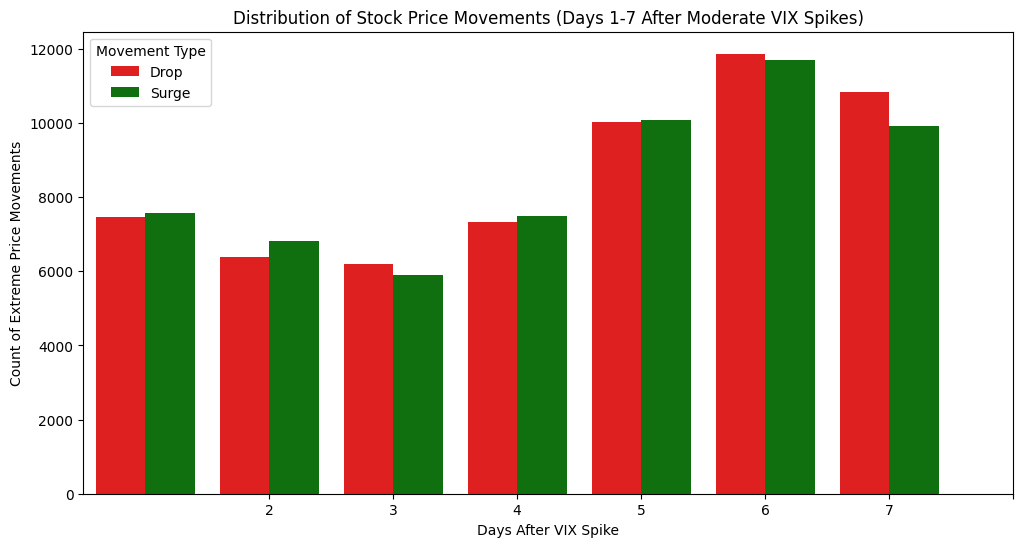
\includegraphics[width=0.5\textwidth]{VIX_correlation_bar_graphs.png}
    \caption{Distribution of Stock Price Movements (Days 1--7 After Moderate VIX Spikes).}
    \label{fig:vix-lag-impact}
\end{figure}

These observations showed promising results, so we decided to move forward with VIX modeling and use these future VIX values as a feature of the overall risk score.

\subsection{Time Series Modeling}

\subsubsection*{Data Preparation and Aggregation}

We split the VIX dataset into 70\% training, 15\% validation, and 15\% test and modeled the following VIX aggregations:

\begin{itemize}
    \item Daily VIX values
    \item Weekly Mean (average of the week)
    \item Weekly Close (last trading day of the week)
\end{itemize}

The VIX dataset was daily from the start so we decided to use it as is. We were concerned from the extra noise we'd get by using the data at such a granular level, so we added 2 additional aggregations, Weekly Mean and Weekly Close. With this we began the time series modeling.

\subsubsection*{Stationarity Testing}

Before we're able to model we have to ensure the data is stationary. This involved visual inspection of the time series and ACF/PACF plots as well as performing the Augmented Dickey-Fuller (ADF) test for stationarity. 

\begin{figure}[h!]
    \centering
    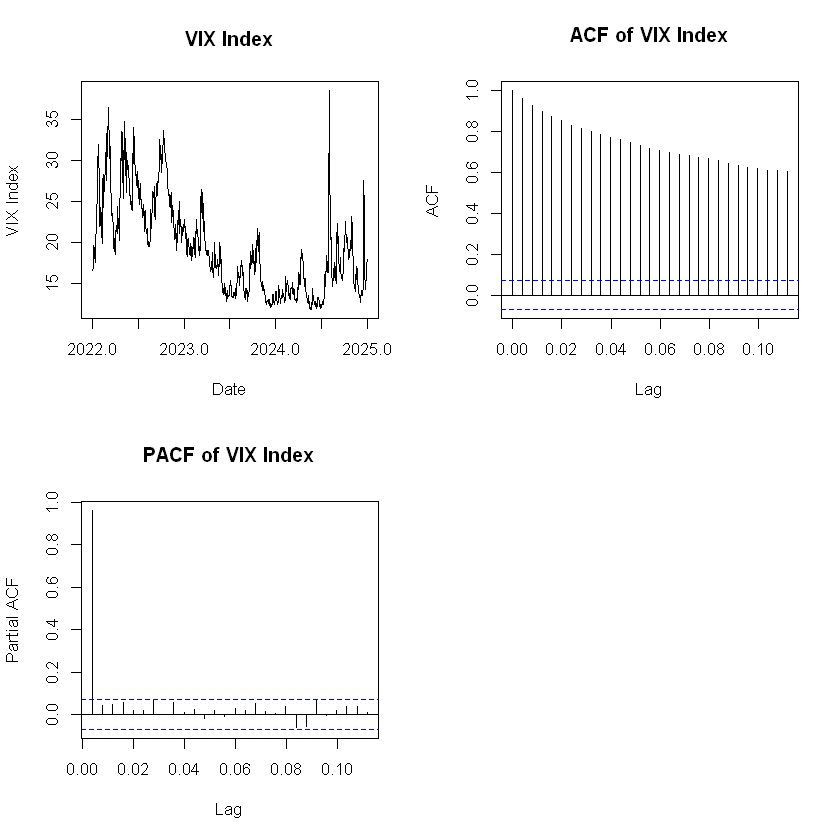
\includegraphics[width=0.5\textwidth]{vix_daily_visual_inspection.png}
    \caption{VIX Daily Close graphs.}
    \label{fig:vix-daily-visual-inspection}
\end{figure}

\begin{figure}[h!]
    \centering
    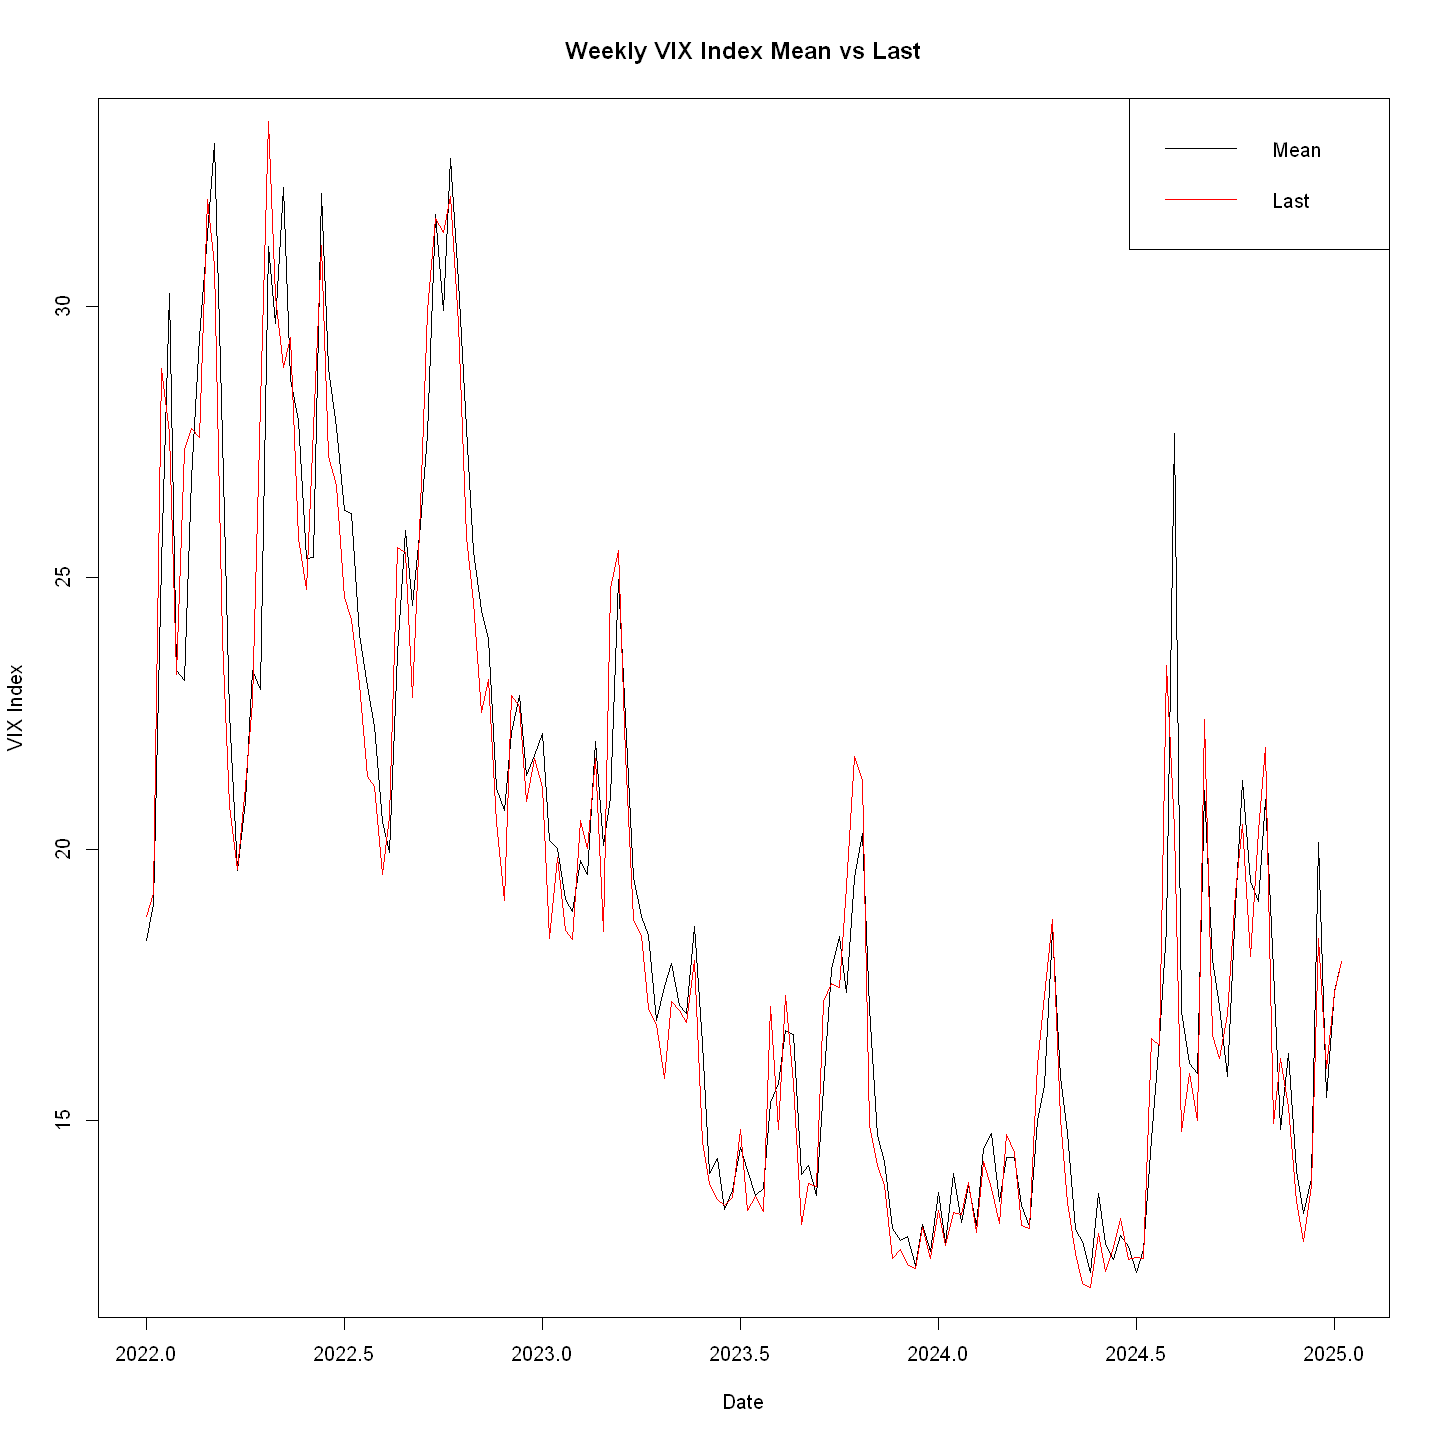
\includegraphics[width=0.5\textwidth]{vix_mean_vs_close_graph.png}
    \caption{VIX Weekly Mean and Weekly Close (shown as Last here) graphs overlaid.}
    \label{fig:vix-weekly-mean-visual-inspection}
\end{figure}


All of the datasets show a downward trend and seasonality so we differenced the data and ensured they passed the ADF test for stationarity.

\subsubsection*{ARIMA Modeling Results}

Once the data was stationary, we moved on towards capturing the model with ARIMA. We iterated over different p, d, and q values, choosing the ones that minimized AICc. We eventually landed on the values seen in table \ref{tab:vix-arima-results}.

\begin{table}[h!]
\centering
\small
\begin{tabular}{|l|c|c|c|}
\hline
\textbf{Dataset} & \textbf{p} & \textbf{q} & \textbf{d} \\
\hline
Weekly Mean & 3 & 5 & 1 \\
Weekly Close & 4 & 3 & 1 \\
Daily VIX & 5 & 4 & 1 \\
\hline
\end{tabular}
\caption{Best p, q, and d values for ARIMA(p,d,q).}
\label{tab:vix-arima-results}
\end{table}

When it came to predictions, we received underwhelming results form this. Table \ref{tab:arima-metrics} has the results.

\begin{table}[h!]
\centering
\small
\begin{tabular}{|l|c|c|c|c|}
\hline
\textbf{Model} & \textbf{MAPE} & \textbf{PM} & \textbf{RMSE} & \textbf{MAE} \\
\hline
Weekly Mean & 8.59 & 1.05 & 1.49 & 1.23 \\
Weekly Close & 9.45 & 0.99 & 1.76 & 1.38 \\
Daily VIX & 9.35 & 2.30 & 3.55 & 2.81 \\
\hline
\end{tabular}
\caption{ARIMA prediction metrics.}
\label{tab:arima-metrics}
\end{table}

The Weekly Mean performed best on all the metrics except for the Precision Error (PM). We believe this is because we smoothed out the data with the Weekly Mean aggregation. Performing an LJung-Box Squared test showed that there was volatility in our data, so using a GARCH model to capture it would be helpful.

\subsubsection*{ARMA-GARCH Modeling}

To find the best model efficiently and without large amounts of nested iterations, we used a heuristic approach to find the best p, q, m, and n for ARMA(p,q)~GARCH(m,n). The approach is as follows:
\begin{enumerate}
    \item Optimize $p$, $q$ for ARMA.
    \item Tune $m$, $n$ for GARCH using fixed ARMA.
    \item Re-tune ARMA based on best GARCH.
    \item Select best model by lowest BIC.
\end{enumerate}

Best model configurations are shown in table \ref{tab:garch-values}. Interestingly enough, the "best" GARCH model for the Daily VIX value didn't involve any GARCH values. Similarly, the best GARCH model for Weekly Mean was a GARCH only model. The only model that used both ARMA and GARCH was the Weekly Close. This is interesting because we assumed that if any of the models wouldn't have a GARCH value, it'd be the smoothened out Weekly Mean model.

\begin{table}[h!]
\centering
\small
\begin{tabular}{|l|c|c|c|c|}
\hline
\textbf{Dataset} & \textbf{p} & \textbf{q} & \textbf{m} & \textbf{n} \\
\hline
Weekly Mean & 0 & 0 & 1 & 1 \\
Weekly Close & 2 & 2 & 0 & 1 \\
Daily VIX & 5 & 4 & 0 & 0 \\
\hline
\end{tabular}
\caption{GARCH configurations.}
\label{tab:garch-values}
\end{table}

The resulting performance is seen in table \ref{tab:garch-metrics}. Both Weekly Close and Daily VIX performed much better than before, while Weekly Mean performed much much worse than its ARIMA counterpart.

\begin{table}[h!]
\centering
\small
\begin{tabular}{|l|c|c|c|c|}
\hline
\textbf{Model} & \textbf{MAPE} & \textbf{PM} & \textbf{RMSE} & \textbf{MAE} \\
\hline
Weekly Mean & 16.50 & 4.38 & 3.04 & 2.33 \\
Weekly Close & 8.41 & 0.75 & 1.54 & 1.20 \\
Daily VIX & 7.82 & 1.96 & 3.28 & 2.37 \\
\hline
\end{tabular}
\caption{GARCH metrics.}
\label{tab:garch-metrics}
\end{table}

\subsection{Classifying Price Movements}

Following our VIX time series modeling, we used the predicted VIX values ($t+7$) to classify future price movements into multiple categories. We experimented with three approaches using XGBoost classifiers, each with different threshold definitions for price fluctuations.

\subsubsection*{3-Class Model}

Our initial approach was a 3-class model that classified the data into the following 3 targets:
\begin{itemize}
    \item $-1$: Drop (price decreased by 2.5\% or more)
    \item $0$: No significant change (between $-2.5\%$ and $2.5\%$)
    \item $1$: Surge (price increased by 2.5\% or more)
\end{itemize}

Since we observed a delayed effect from the VIX, we used the lagged price and volume features over a 7-day window. The features used were:

\texttt{ticker, subindustry, VIX\_t, VIX\_t-7, VIX\_t+7**, positive/neutral/negative sentiment scores, top sentiment label, lagged price, price \% change, lagged volume, and volume \% change}

**We trained the model using observed VIX at $t+7$ during training, but during prediction, we substituted this with our predicted VIX value. 

The model performed \textit{a little too well} with an accuracy of 100\%.

\begin{table}[h!]
\centering
\small
\begin{tabular}{|l|c|c|c|c|}
\hline
\textbf{label} & \textbf{precision} & \textbf{recall} & \textbf{f1-score} \\
\hline
           -1    &   0.98    &   0.99   &    0.99    \\
            0    &    1.00   &    1.00  &     1.00    \\ 
            1    &    0.98   &    1.00   &    0.99    \\
\hline
\end{tabular}
\caption{3 class classifier metrics.}
\label{tab:3-class-metrics}
\end{table}


We noticed that there was a huge class imbalance. The distribution is shown in table \ref{tab:3-class-distribution}.

\begin{table}[h!]
\centering
\small
\begin{tabular}{|c|c|}
\hline
\textbf{label} & \textbf{distribution} \\
\hline
  0   & 169,018 \\
  1   &  16,569 \\ 
 -1   &  15,480 \\ 
\hline
\end{tabular}
\caption{3 class classifier distribution.}
\label{tab:3-class-distribution}
\end{table}

Despite the strong metrics, the model overwhelmingly predicted class 0. To address this, we introduced more granular classes.

\subsubsection*{5-Class Model}

We adjusted our thresholds to define 5 distinct classes:

\begin{table}[h!]
\centering
\small
\begin{tabular}{|c|c|c|}
\hline
\textbf{Class} & \textbf{\% price movement} & \textbf{Description} \\
\hline
-2 & $\leq -5.0\%$ & Huge Drop  \\
-1 & $> -5.0\%$ and $\leq -2.5\%$ & Moderate Drop  \\
 0 & $> -2.5\%$ and $\leq 2.5\%$ & No Change \\
 1 & $> 2.5\%$ and $\leq 5.0\%$ & Moderate Surge  \\
 2 & $> 5.0\%$ & Major Surge  \\
\hline
\end{tabular}
\caption{5 class classifier labels.}
\label{tab:5-class-labels}
\end{table}

This balanced the class distribution some more but didn't get rid of the giant cluster at "No Change" label 0.

\begin{table}[h!]
\centering
\small
\begin{tabular}{|c|c|}
\hline
\textbf{label} & \textbf{distribution} \\
\hline
  0  &   165,338 \\
  1  &    12,500 \\
 -1  &    11,285 \\
 -2  &     4,066 \\
  2  &     3,837 \\
\hline
\end{tabular}
\caption{5 class classifier labels.}
\label{tab:5-class-distribution}
\end{table}

To compensate for this imbalance, we added class weights to the XGBoost model. This improved the performance and resulted in predictions that were better spread across classes as seen in table \ref{tab:5-class-metrics}. Our accuracy dropped a bit from the previous model to 90\%.

\begin{table}[h!]
\centering
\small
\begin{tabular}{|l|c|c|c|c|}
\hline
\textbf{label} & \textbf{precision} & \textbf{recall} & \textbf{f1-score} \\
\hline
             -2    &   0.89  &    0.48  &    0.63  \\
             -1    &   0.55  &    0.09  &    0.15  \\
              0    &   0.91  &    0.99  &    0.95  \\
              1    &   0.74  &    0.31  &    0.44  \\
              2    &   0.82  &    0.34  &    0.48  \\
\hline
\end{tabular}
\caption{5 class classifier metrics. \textbf{\textit{Note:}} While it is not shown, we shifted all labels by +2 to fit XGBoost’s label constraints (i.e., no negative class labels).}
\label{tab:5-class-metrics}
\end{table}
        % accuracy                           0.90     24898
% \end{verbatim}


The most important feature based on feature importance was the predicted VIX at $t+7$, further reinforcing its predictive value.

%% figure!
\begin{figure}[h!]
    \centering
    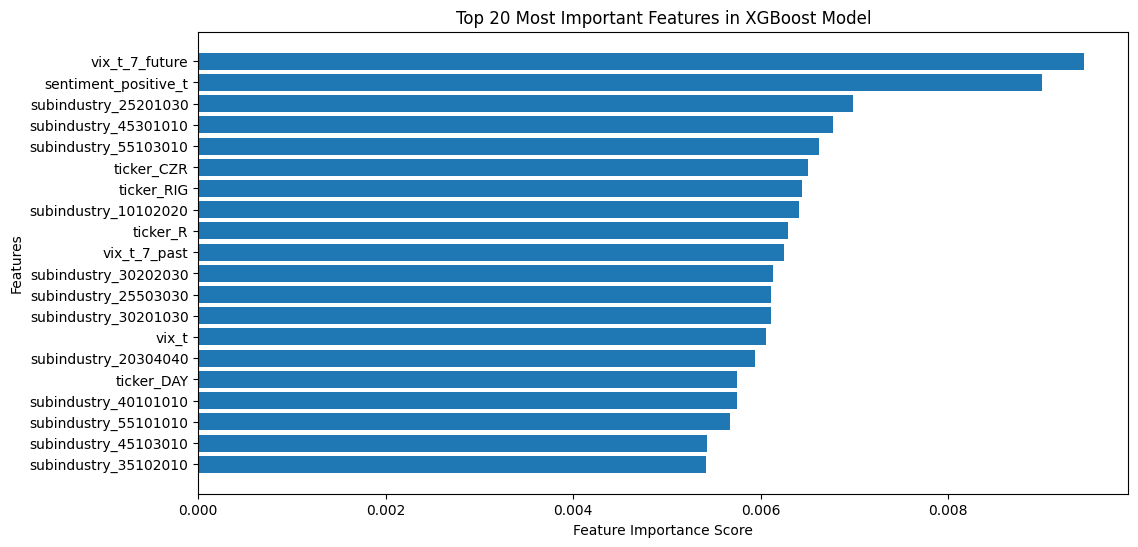
\includegraphics[width=0.45\textwidth]{5_class_xgboost_important_features.png}
    \caption{Top 20 features ordered by importance in XGBoost.}
    \label{fig:5-class-feature-importance}
\end{figure}


\subsubsection*{7-Class Model}

To further split the dominant “no change” bucket, we tried a 7-class setup:

\begin{table}[h!]
\centering
\small
\begin{tabular}{|c|c|c|}
\hline
\textbf{Class} & \textbf{\% price movement} & \textbf{Description} \\
\hline
-2 & $\leq -5.0\%$ & Huge Drop  \\
-1 & $> -5.0\%$ to $\leq -2.5\%$ & Moderate Drop  \\
 0 & $> -2.5\%$ to $\leq -0.5\%$ & Minor Drop \\
 1 & $> -0.5\%$ to $\leq 0.5\%$ & No Change  \\
 2 & $> 0.5\%$ to $\leq 2.5\%$ & Minor Surge  \\
 3 & $> 2.5\%$ to $\leq 5.0\%$ & Moderate Surge  \\
 4 & $> 5.0\%$ & Major Surge  \\
\hline
\end{tabular}
\caption{7 class classifier labels. No change is now label 1 in this setup.}
\label{tab:7-class-labels}
\end{table}


This produced a more balanced distribution as seen in table \ref{tab:7-class-distribution}

\begin{table}[h!]
\centering
\small
\begin{tabular}{|c|c|}
\hline
\textbf{label} & \textbf{distribution} \\
\hline
   1  &  69,672 \\
   2  &  52,050 \\
   0  &  43,616 \\
   3  &  12,500 \\
  -1  &  11,285 \\
  -2  &   4,066 \\
   4  &   3,837 \\
\hline
\end{tabular}
\caption{7 class classifier labels.}
\label{tab:7-class-distribution}
\end{table}

Performance:

\begin{table}[h!]
\centering
\small
\begin{tabular}{|l|c|c|c|c|}
\hline
\textbf{label} & \textbf{precision} & \textbf{recall} & \textbf{f1-score} \\
\hline
               -2   &    0.87  &    0.52  &    0.65 \\
               -1   &    0.67  &    0.20  &    0.30 \\
               0   &    0.56  &    0.22  &    0.32 \\
               1   &    0.41  &    0.69  &    0.51 \\
               2   &    0.48  &    0.46  &    0.47 \\
               3   &    0.72  &    0.40  &    0.51 \\
               4   &    0.83  &    0.36  &    0.50 \\
\hline
\end{tabular}
\caption{7 class classifier metrics. As before we applied a +2 shift to the labels which is not shown in the above table.}
\label{tab:7-class-metrics}
\end{table}
        %       precision    recall  f1-score   support
        % accuracy                           0.46     24898

While the overall accuracy dropped to 46\%, we were able to capture more price movement variation and break up the large "No Change" cluster. 
While we retained a high precision and recall for the extreme cases (labels -2 and 4), the model struggled more with subtler price movements as seen in the lower precision and recall scores for those intermediate labels. 

This highlights the benefits of class weighting with underrepresented classes. It was less effective for the middle categories where they had more data but where still overshadowed by the "No Change" cluster.

\subsubsection*{Conclusion}

Across all models, class imbalance proved to be the primary challenge. The 3-class model had high scores but was overly biased toward the dominant “No Change” class. The 5-class model struck a better balance and showed promise, especially with class weighting. The 7-class model, while less accurate, offered more realistic and nuanced results by capturing subtler movements. 

Unfortunately, none of the aforementioned models brought much confidence due to the data imbalance that we had. They'd be great at predicting "No Change" signals, which isn't the goal of this project.

We also experimented with logistic regression and decision trees, but none outperformed XGBoost across these multi-class setups. Based on feature importance, the predicted VIX value at $t+7$ was consistently the most significant input in all models.

%%%%%%%%%%%%%%%%%%%%%%%%%%%%%%%%%%%%%%%%%%%%%%%%%%%%%%%%%%%%%%%%%%%%%%%%%%%%%%
%%%%%%%%%%%%%%%%% Adding Word Embedding and Clustering  %%%%%%%%%%%%%%%%%%%%%%
%%%%%%%%%%%%%%%%%%%%%%%%%%%%%%%%%%%%%%%%%%%%%%%%%%%%%%%%%%%%%%%%%%%%%%%%%%%%%%
\section{Thematic Clustering}
To explore alternative approaches to labeling sentiment in financial news, we developed an unsupervised clustering pipeline using Word2Vec embeddings and the Loughran-McDonald (LM) financial lexicon. This approach was inspired by the text summarization approach done by Haider et al.~\cite{9230670} Due to the short text information from the articles and complex relationships within the market, we decided to modify their approach to use density based clustering instead of K-means. Additionally we used a combination of metrics to find the best Word2Vec paramaters that maximized the vector information. This allowed us to rely on unseen relationships between the articles to label the thematic category of article clusters using the LM lexicon.

\subsubsection*{Embedding Financial News Articles}

We first cleaned and tokenized article titles and descriptions by removing punctuation, stopwords, and irrelevant tokens. A custom Word2Vec Skip-Gram model was then trained on the cleaned corpus. To validate the quality of our embeddings, we compared them against the WordSim-353 benchmark using Spearman correlation, as discussed by Kliegr and Zamazal \cite{KLIEGR2018174}, and achieved a coefficient of 0.2568 with:
\begin{itemize}
    \item \texttt{vector\_size} = 400
    \item \texttt{window} = 4
\end{itemize}

We then averaged the word embeddings in each article to obtain a document vector representing its semantic content.

\subsubsection*{Clustering with DBSCAN and HDBSCAN}

We applied two density-based clustering methods: DBSCAN and HDBSCAN, both of which are well-suited for discovering non-spherical clusters and identifying noise.

\textbf{DBSCAN}: We tuned DBSCAN’s eps and min samples parameters using Silhouette Score, Davies-Bouldin Score, cluster count, and noise ratio. The best configuration was:
\begin{itemize}
    \item \texttt{eps} = 1.2
    \item \texttt{min\_samples} = 50
    \item Result: ~19 clusters (including noise)
\end{itemize}

\begin{figure}[h!]
    \centering
    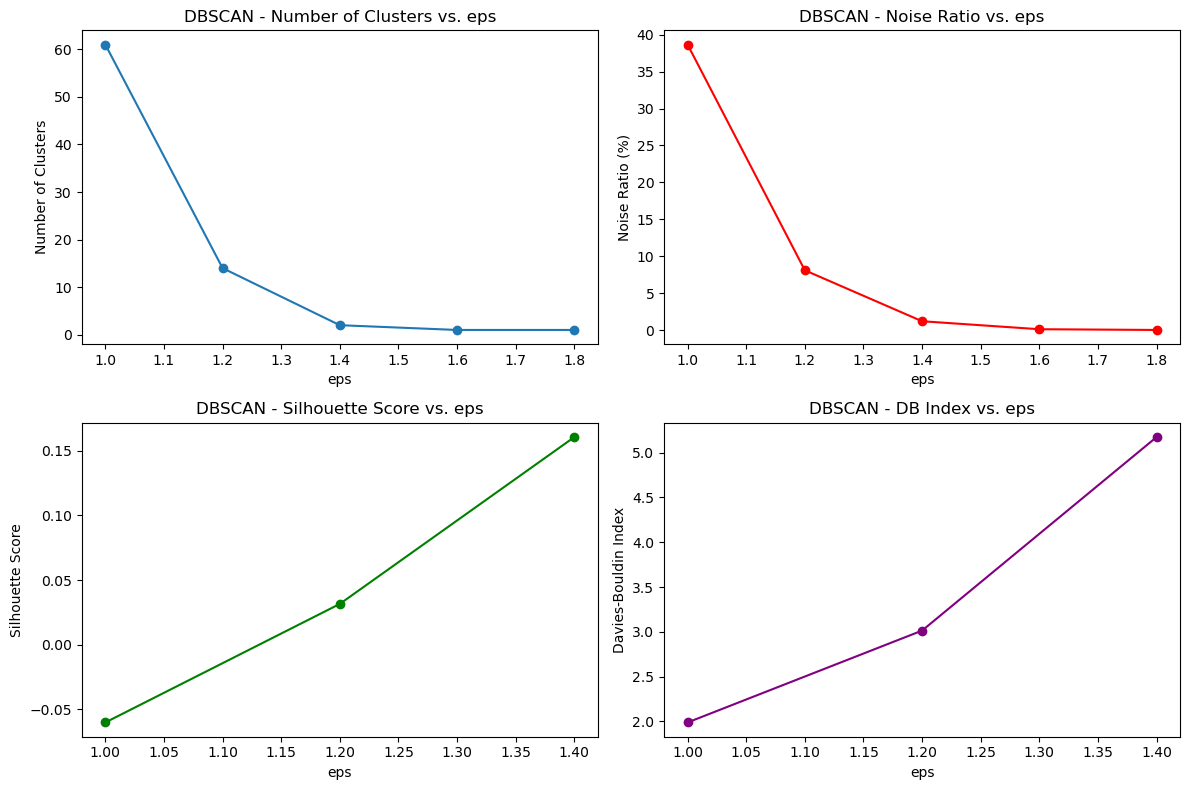
\includegraphics[width=0.49\textwidth]{DBSCAN_tuning_metrics.png}
    \caption{DBSCAN tuning metrics.}
    \label{fig:dbscan-tuning}
\end{figure}


Unfortunately, we observed a large class imbalance, with one dominant cluster as seen in figure \ref{fig:dbscan-high-cluster}. We applied sub-clustering to the largest group using eps = 1.0 and min samples = 37, which resulted in 46 additional subclusters as seen in figure \ref{fig:dbscan-subcluster}. However, this recursive process still failed to fully resolve imbalance. To prevent doing this recursively until we finally break up the dominant cluster, we decided to see what information we can get from just one level of clustering.

\begin{figure}[h!]
    \centering
    \begin{subfigure}[t]{0.49\textwidth}
        \centering
        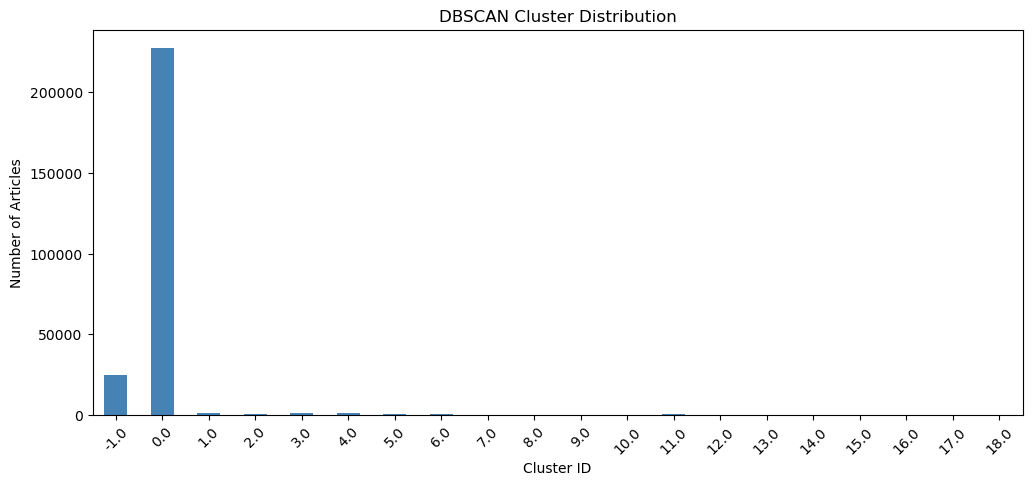
\includegraphics[width=\textwidth]{dbscan_distribution.png}
        \caption{DBSCAN after clustering.}
        \label{fig:dbscan-high-cluster}
    \end{subfigure}
    \hfill

    \begin{subfigure}[t]{0.49\textwidth}
        \centering
        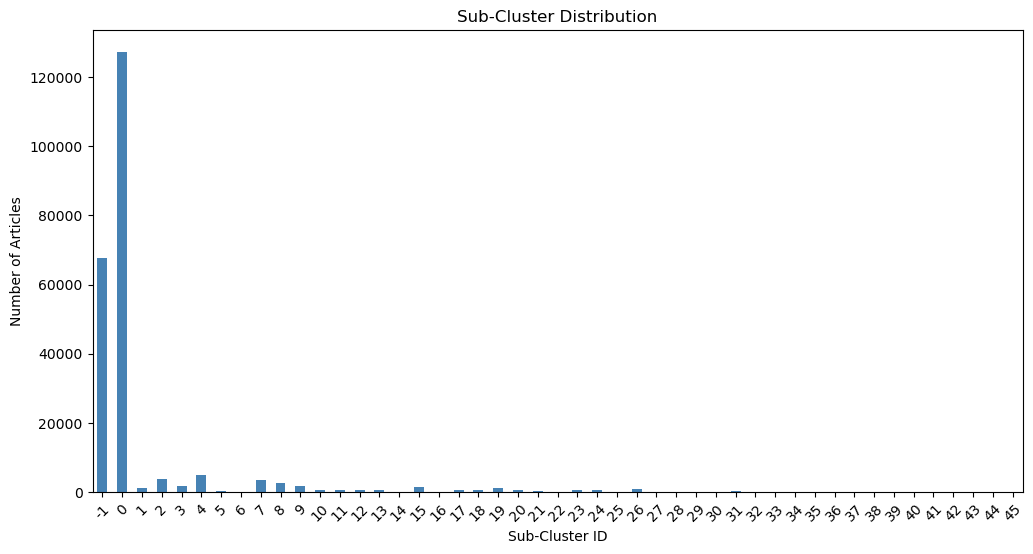
\includegraphics[width=\textwidth]{dbscan subcluster.png}
        \caption{DBSCAN after sub-clustering.}
        \label{fig:dbscan-subcluster}
    \end{subfigure}
    \hfill
    \begin{subfigure}[t]{0.49\textwidth}
        \centering
        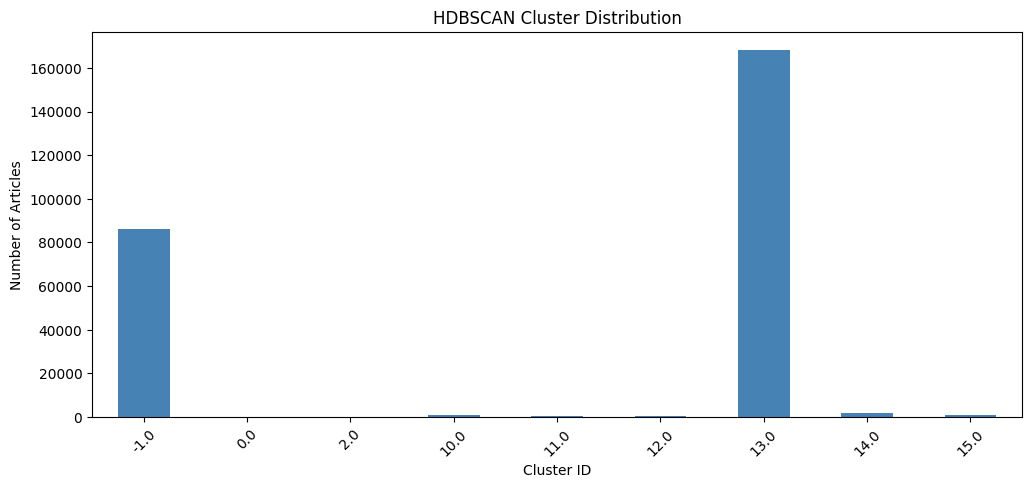
\includegraphics[width=\textwidth]{HDBSCAN_subcluster_distribution.png}
        \caption{HDBSCAN after sub-clustering.}
        \label{fig:hdbscan-subcluster}
    \end{subfigure}


    \caption{DBSCAN and HDBSCAN cluster distribution. -1 denotes the noise cluster.}
    \label{fig:dbscan-both}
\end{figure}



\textbf{HDBSCAN}:  
We faced many challenges trying to implement this clustering algorithm due to its heavy CPU limitations. HDBSCAN was initially abandoned but was later revisited using a GPU-accelerated version via NVIDIA’s cuML library\cite{sharma2025nvidia}. 

This approach yielded 4 main clusters (including noise). Similar to DBSCAN, we achieved one extremely dominant cluster and several smaller ones. Further sub-clustering produced 9 total clusters but did not fully break up the dominant cluster as seen in figure \ref{fig:hdbscan-subcluster}.

\subsubsection*{Labeling Clusters with Risk Sentiment}

To assign a thematic sentiment to each cluster, we used the LM financial lexicon to tag clusters with sentiment categories:
\begin{itemize}
    \item Positive
    \item Negative
    \item Litigious
    \item Uncertain
    \item Mixed Sentiment (default when no category dominated)
\end{itemize}

Each cluster was labeled based on the proportion of its vocabulary overlapping with lexicon categories. We used a multi-labeling approach to capture mixed risk types. Below are examples of labeled clusters from each algorithm:

\textbf{DBSCAN Cluster Tags} (excerpt):
\begin{itemize}
    \item Cluster 0.0: [Negative, Positive]
    \item Cluster 4.0: [Negative, Positive, Uncertainty]
    \item Cluster 6.0: [Negative, Uncertainty]
    \item Cluster 12.0: [Negative, Uncertainty]
    \item Cluster 15.0: [Positive]
\end{itemize}

\textbf{HDBSCAN Cluster Tags} (excerpt):
\begin{itemize}
    \item Cluster -1.0: [Negative, Positive]
    \item Cluster 2.0: [Negative, Uncertainty]
    \item Cluster 13.0: [Negative, Positive]
    \item Cluster 15.0: [Negative, Positive, Uncertainty]
\end{itemize}

The results were interesting, as some clusters had both negative and positive sentiment. This could mean that the articles in these clusters had both positive and negative news. We know articles could talk about 1 or many tickers at once, so there could be a mix where a ticker has good news but another has negative news within the same article.

\subsubsection*{Comparing DBSCAN vs. HDBSCAN Labeling}

Although clustering was not usable for predictive modeling due to the severe imbalance, we decided to compare the results from both of these attempts.

\begin{figure}[h!]
    \centering
    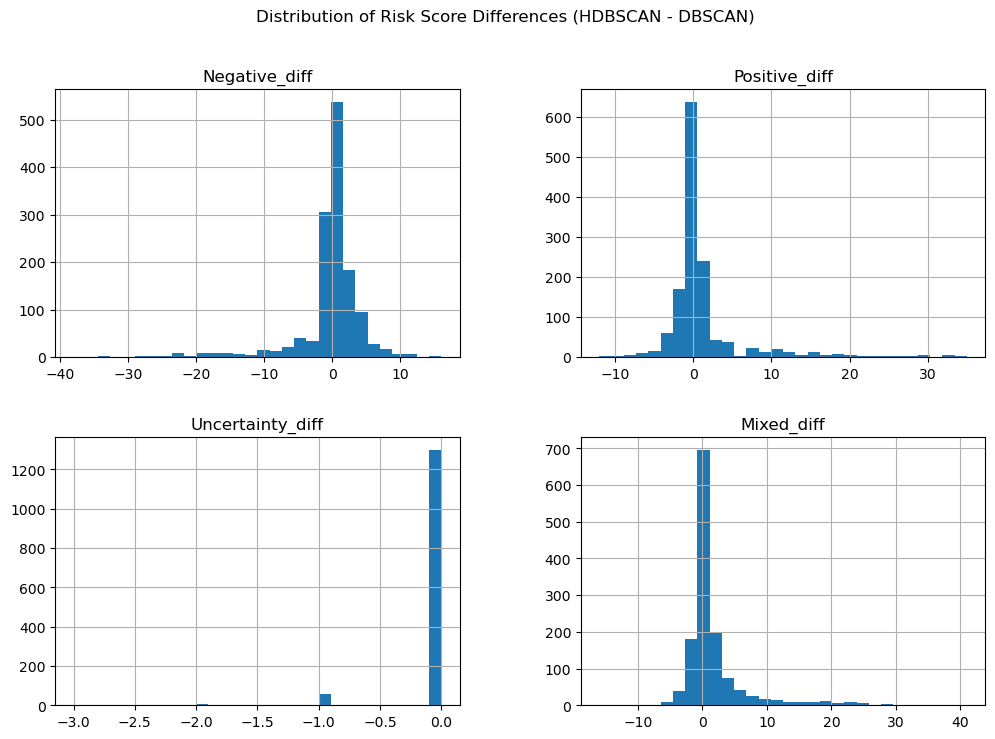
\includegraphics[width=0.49\textwidth]{hdbscan_vs_dbscan.png}
    \caption{HDBSCAN vs DBSCAN.}
    \label{fig:hdbscan-vs-dbscan}
\end{figure}



\textbf{Key Observations:}
\begin{itemize}
    \item \textbf{Negative Sentiment:} DBSCAN assigned more distinct negative clusters shown by the long negative tail. HDBSCAN was more conservative.
    \item \textbf{Uncertainty:} Both methods had nearly identical Uncertainty scores, suggesting consistent identification of uncertain content.
    \item \textbf{Positive Sentiment:} DBSCAN assigned positive tags to more tickers overall, while HDBSCAN had fewer but more distinct positive clusters shown by the long positive tail.
    \item \textbf{Mixed Sentiment:} Both models agreed on mixed sentiment tagging for ambiguous clusters, with HDBSCAN being slightly more liberal in assigning this category.
\end{itemize}

\subsubsection{Clustering with FinBERT Embeddings}


Since the results from our Word2Vec-based clustering (via DBSCAN and HDBSCAN) were somewhat underwhelming, we decided to explore a transformer-based embedding model, FinBERT. We hoped this switch would allow us to capture more contextualized representations of the financial text since this model is pre-trained on a financial corpus.

Compared to Word2Vec, the FinBERT approach was more hands-off. The model handled tokenization, sanitation, and embedding internally, making the pipeline much simpler. For clustering, we used HDBSCAN, which we found to be more effective than DBSCAN for handling variable-density clusters and separating noise.\cite{pratap2023dbscan}

We performed a parameter grid search and identified the best configuration as:
\begin{itemize}
    \item \texttt{min\_cluster\_size} = 150
    \item \texttt{min\_samples} = 100
\end{itemize}
This configuration minimized cluster size while maximizing cluster count, as shown in figure \ref{fig:finbert-tuning}.

\begin{figure}[h!]
    \centering
    \begin{subfigure}[t]{0.49\textwidth}
        \centering
        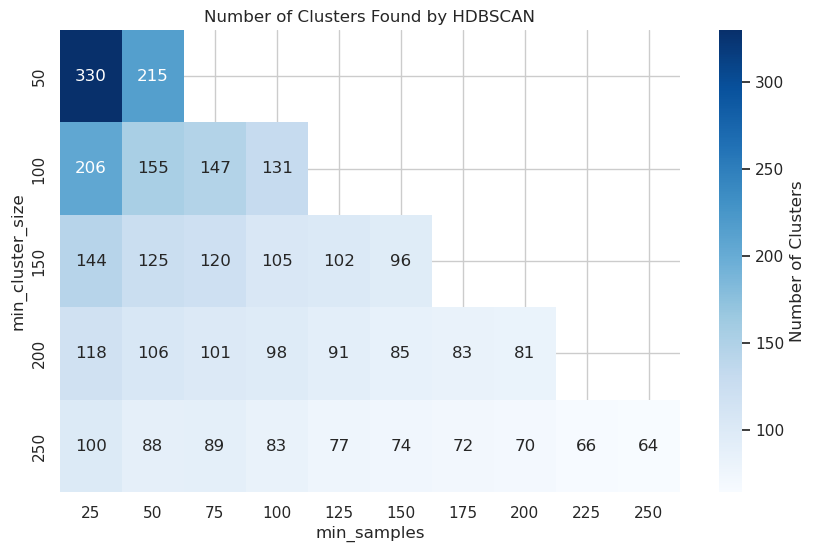
\includegraphics[width=\textwidth]{finbert_hdbscan_clusters.png}
        \caption{Number of FinBERT clusters using HDBSCAN.}
        \label{fig:finbert-cluster-num}
    \end{subfigure}
    \hfill
    \begin{subfigure}[t]{0.49\textwidth}
        \centering
        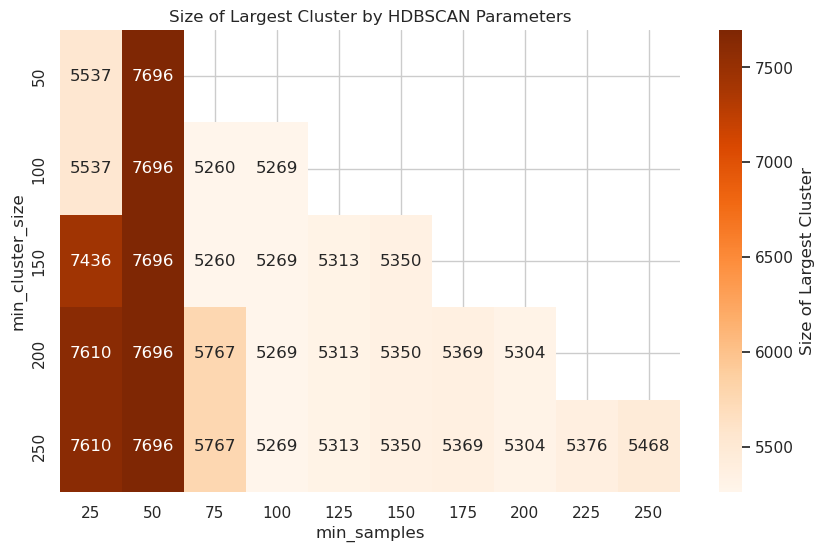
\includegraphics[width=\textwidth]{finbert_hdbscan_largest_cluster.png}
        \caption{Size of largest FinBERT clusters using HDBSCAN.}
        \label{fig:finbert-cluster-size}
    \end{subfigure}


    \caption{HDBSCAN results from grid search hyper parameter tuning.}
    \label{fig:finbert-tuning}
\end{figure}


We then ran the resulting clusters through the same multi-label risk tagging pipeline using the LM lexicon. Surprisingly, the results were the same across all clusters, with the same two labels: \textbf{[Negative, Positive]}.

\textbf{FinBERT HDBSCAN Cluster Tags} (excerpt):
\begin{itemize}
    \item Cluster 0: [Negative, Positive]
    \item Cluster 1: [Negative, Positive]
    \item Cluster 2: [Negative, Positive]
    \item Cluster 9: [Negative, Positive]
\end{itemize}

This result was somewhat ironic, given that FinBERT itself is designed to classify text as either negative, positive, or neutral. We're not sure if this outcome is a byproduct of the transformer architecture or a result of the clustering process. Ultimately this approach did not yield the insights we hoped for because the clusters did not offer meaningful differentiation in terms of risk sentiment.

\subsubsection*{Conclusion}

This clustering pipeline helped uncover thematic risk patterns and offered a new way to use article data past the positive, negative, and neutral tagging done by FinBERT. Despite the class imbalance challenges, the labeling approach provided insight into common themes shared by the articles, proving this could be a reasonable approach at exploring hidden relationships in the complex landscape of financial texts. Unfortunately this was not stable enough to use for the overall risk score, but it was a fun way to explore sentiment analysis.

%%%%%%%%%%%%%%%%%%%%%%%%%%%%%%%%%%%%%%%%%%%%%%%%%%%%%%%%%%%%%%%%%%%%%%
%% Token Word Score and Sentiment Analysis Approach
%%%%%%%%%%%%%%%%%%%%%%%%%%%%%%%%%%%%%%%%%%%%%%%%%%%%%%%%%%%%%%%%%%%%%%
\section{Token Word Score and Sentiment Analysis Approach}
This approach leverages token-level analysis to compute a detailed risk metric from financial news articles. Our focus on sentiment—especially negative tone—and its relationship to volatility is aligned with prior findings in the literature showing that negative language in financial news can forecast lower future returns and increased market volatility~\cite{tetlock2007}.

\subsubsection{Risk Score Computations}

Three distinct risk scores were calculated for each ticker:

\begin{enumerate}
    \item \textbf{Basic Sentiment Risk:} The volatility (standard deviation) of sentiment scores from FinBERT's title and description analyses.
    \item \textbf{Enhanced Sentiment Risk:} Incorporates additional sentiment features, including positive, neutral, and negative scores from both titles and descriptions.
    \item \textbf{Comprehensive Risk:} Combines sentiment volatility, high-risk word count variability, and token score variability into a single measure.
\end{enumerate}

Correlation analysis (Figure~\ref{fig:risk_corr_heatmap}) and regression results (Figure~\ref{fig:risk_regressions}) highlight that the Comprehensive Risk measure has the strongest relationship with stock volatility (correlation: 0.58, R$^2$: 0.33), significantly outperforming the Basic (R$^2$: 0.06) and Enhanced Sentiment Risk (R$^2$: 0.02) measures. This indicates that combining sentiment, high-risk words, and token-level variability offers greater predictive insight into volatility.

\begin{figure}[ht]
    \centering
    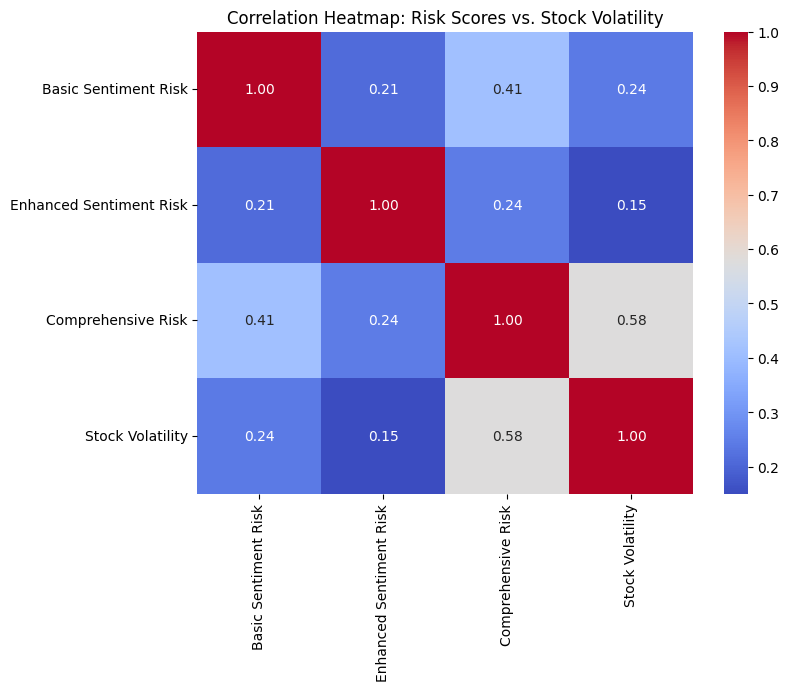
\includegraphics[width=0.5\textwidth]{correlation_heatmap_risks.png}
    \caption{Correlation Heatmap of Risk Scores and Stock Volatility.}
    \label{fig:risk_corr_heatmap}
\end{figure}

\begin{figure}[ht]
    \centering
    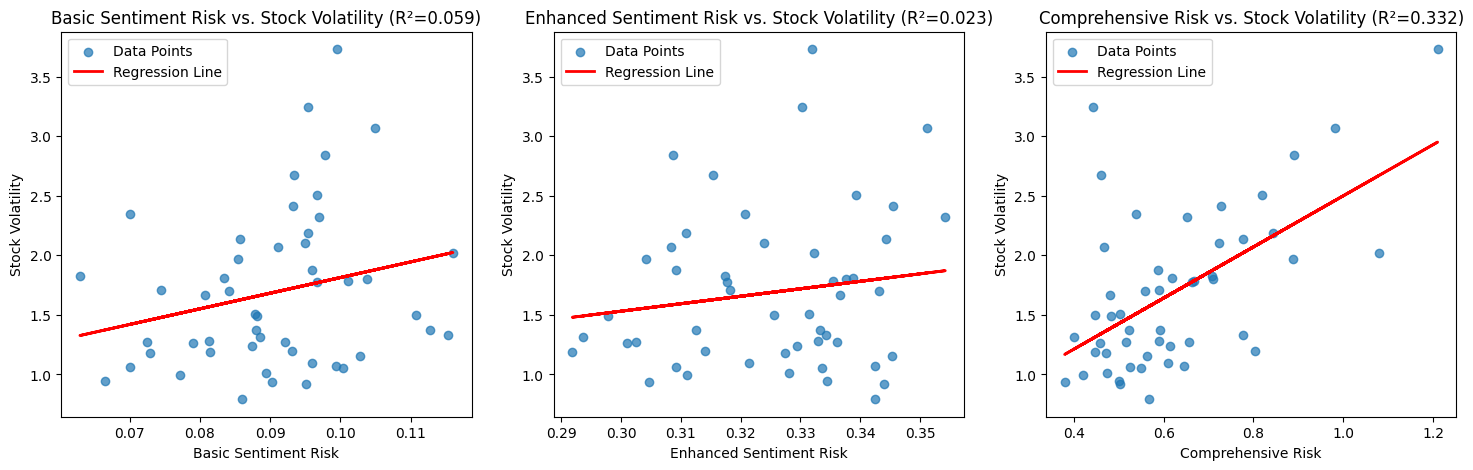
\includegraphics[width=0.5\textwidth]{regression_risk_volatility.png}
    \caption{Regression Analysis of Risk Scores versus Stock Volatility.}
    \label{fig:risk_regressions}
\end{figure}

\subsubsection{Weighted Risk Score Experiments}

To identify the most effective weighting strategy, we experimented with multiple schemes:

\begin{itemize}
    \item \textbf{Equal Weights:} Equal contribution of sentiment volatility, high-risk words, and token variability.
    \item \textbf{Sentiment-Focused:} Greater emphasis on sentiment volatility (60\%).
    \item \textbf{High-Risk-Focused:} Greater emphasis on high-risk word variability (60\%).
    \item \textbf{Token-Focused:} Greater emphasis on token-level variability (60\%).
\end{itemize}

The correlation heatmap (Figure~\ref{fig:weighted_risk_heatmap}) indicates that the Token-Focused Risk strongly correlates with stock volatility (correlation: 0.65), outperforming other weighting schemes. This suggests that token-level granularity captures substantial volatility signals.

\begin{figure}[ht]
    \centering
    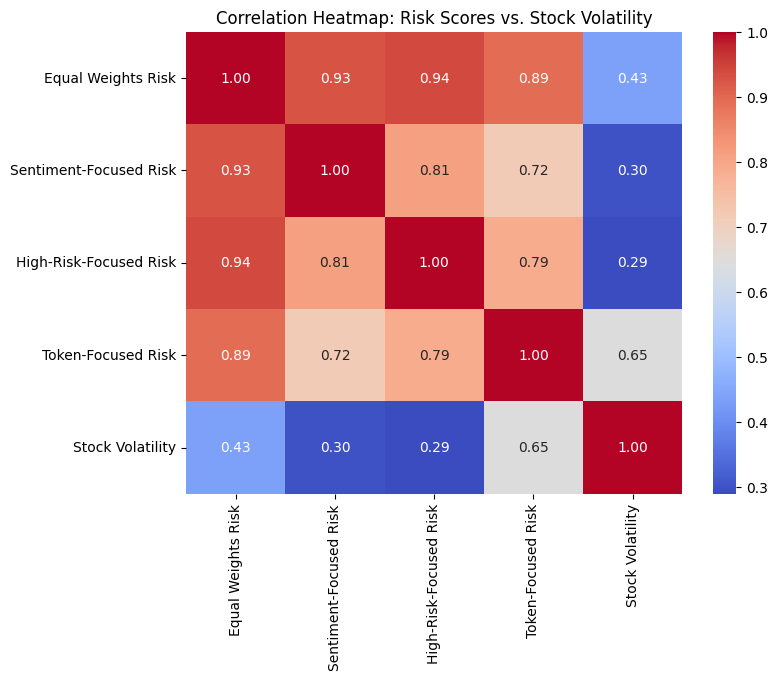
\includegraphics[width=0.5\textwidth]{weighted_risk_heatmap.png}
    \caption{Correlation Heatmap of Weighted Risk Scores and Stock Volatility.}
    \label{fig:weighted_risk_heatmap}
\end{figure}

\subsubsection{Key Insights}

The analysis underscores several important findings:
\begin{itemize}
    \item Combining multiple sentiment and token-based features significantly improves volatility prediction compared to using sentiment alone.
    \item Token-focused approaches show the greatest promise, emphasizing the critical role of detailed textual analysis at the token level.
    \item Weighted combinations of risk measures provide additional insights, offering opportunities for customized volatility modeling.
\end{itemize}

\subsection{Multi-Feature vs. Token-Focused Models}

\subsubsection{Multi-Feature Model (11 Features Including \texttt{article\_count})}

This model utilized a comprehensive set of features, including sentiment scores (from FinBERT), token-based indicators (e.g., token-level sentiment scoring and high-risk word counts), and metadata such as the number of articles per ticker. While the inclusion of diverse features aimed to improve generalization, the model's performance varied widely across tickers.

\textbf{Important Note on Interpretation:}  
While the $R^2$ metric is theoretically bounded above by 1.0, our analysis observed several ticker-specific models producing $R^2$ values exceeding this limit. These inflated values stem from a combination of factors:
\begin{itemize}
    \item Extremely small test set sizes for certain tickers, leading to unstable variance estimates.
    \item Outliers in price change percentages skewing performance metrics.
    \item Model overfitting on sparse or noisy feature combinations.
\end{itemize}

\begin{itemize}
    \item \textbf{Median $R^2$ Scores (across 50 tickers):}
    \begin{itemize}
        \item \textbf{XGBoost:} 1.06
        \item \textbf{Linear Regression:} 1.07
        \item \textbf{Random Forest and Neural Network:} Generally lower, often negative or highly variable.
    \end{itemize}
\end{itemize}

\textbf{Additional Observations:}
\begin{itemize}
    \item The mean $R^2$ scores were highly skewed by outlier values, reaffirming the use of the \textbf{median} as a more stable indicator of overall model performance.
    \item Despite the richness of the feature set, models often overfit—especially when article volume was low or sentiment features lacked variability.
\end{itemize}

These findings motivated us to streamline our modeling pipeline. In the following section, we explore a simplified, token-focused feature—derived from sentiment scores, high-risk word counts, and token scoring—that achieved more stable and generalizable results with lower variance in both $R^2$ and MAE.


\subsubsection{Token-Focused Model (Single Feature: \texttt{token\_focused\_risk})}
This model was streamlined, employing a single engineered feature that aggregated sentiment scores, high-risk word counts, and token-level risk metrics:

\begin{itemize}
    \item \textbf{Median $R^2$ Scores:}
    \begin{itemize}
        \item \textbf{XGBoost:} 0.75
        \item \textbf{Linear Regression:} 0.70
        \item \textbf{Neural Network and Random Forest:} Also showed consistent and stable performance.
    \end{itemize}
    \item \textbf{Observations:}
    \begin{itemize}
        \item Demonstrated greater stability and fewer outliers.
        \item Proved that a well-designed single feature can deliver robust predictive performance, reducing the risk of overfitting.
    \end{itemize}
\end{itemize}

\subsection{Impact of Article Count on Model Performance}
Implementing a minimum article threshold (100 articles per ticker) significantly reduced noise and enhanced reliability of performance metrics:

\begin{itemize}
    \item Including \texttt{article\_count} explicitly as a feature further improved explanatory power.
    \item These findings were consistent with prior topic-modeling experiments, emphasizing the critical role of adequate article volume.
\end{itemize}

\subsection{Key Insights and Recommendations}

\begin{enumerate}
    \item \textbf{Simplicity enhances model robustness:} The token-focused risk feature alone effectively captured significant predictive insights.
    \item \textbf{Median metrics provide more stable information:} Median values were more indicative of true model performance compared to mean values due to outlier influence.
    \item \textbf{Article volume is essential:} Providing enough data per ticker improved both the accuracy and reliability of the model.
    \item \textbf{Model sensitivity to noise:} Random Forests and Neural Networks exhibited high sensitivity to noisy data without hyperparameter tuning, indicating a need for cautious selection or further optimization.
\end{enumerate}

%%%%%%%%%%%%%%%%%%%%%%%%%%%%%%%%%%%%%%%%%%%%%%%%%%%%%%%%%%%%%%%%%%%%%%
%% Alternate risk score, technical anlaysis, NER
%%%%%%%%%%%%%%%%%%%%%%%%%%%%%%%%%%%%%%%%%%%%%%%%%%%%%%%%%%%%%%%%%%%%%%

\section{Alternative Risk Score Method with Named Entity Recognition and Technical Analysis}
This method focuses on a weighted score with NER reduced token words. We also studied the impact on the performance of the model by adding additional features such as VIX and technical indicators.

\subsection{Risk Score Calculation Steps:}
\begin{enumerate}
    \item \textbf{Tokenization:} Articles are cleaned, tokenized, and lemmatized. Stopwords and non-informative tokens are removed.
    \item \textbf{NER removal:} Run spaCy's named entity recognition function to remove all NER from tokenized words.
    \item \textbf{Final Set:} find set of all tokenized words(NER removed) to remove duplicate words.
    \item \textbf{Calculate risk score for each tokenized word:} 
    \begin{enumerate}
    \item \textbf{Iterate thru each trading day and add weighted score to each word in the final set.}
    \item \textbf{The weighted score for each trading day for a particular word = total appearance of that word/total word count * tomorrow's stock increase percentage.}
    \item \textbf{risk score for particular word = total weighted score sum / total trading days.}
    \end{enumerate}
    \begin{figure}[ht]
        \centering
        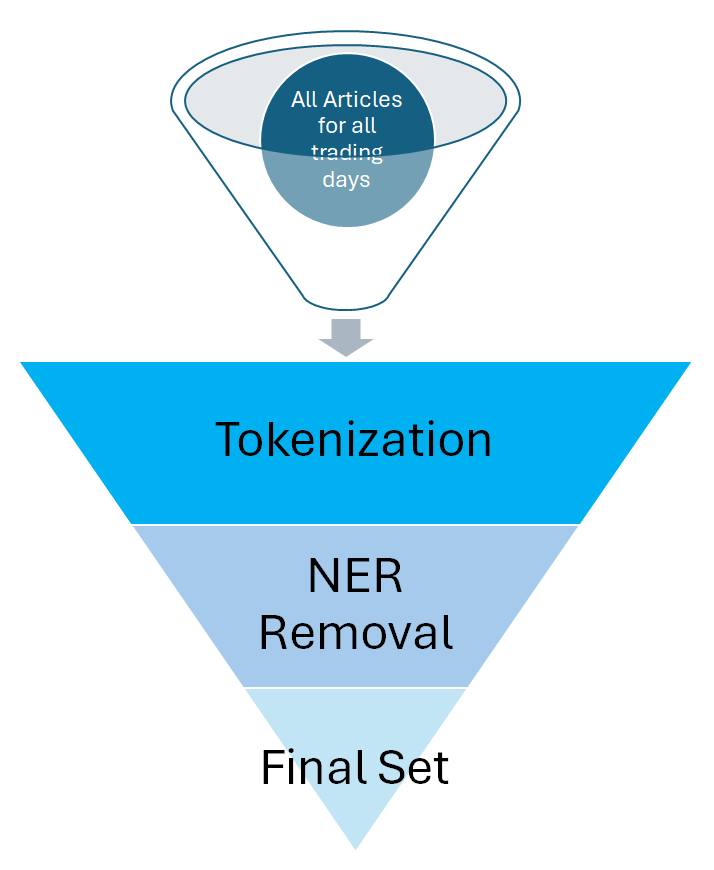
\includegraphics[width=0.5\textwidth]{Token_word_set.png}
        \caption{Tokenization and Reduction.}
        \label{fig:tonkenization}
    \end{figure}
    \begin{figure}[ht]
        \centering
        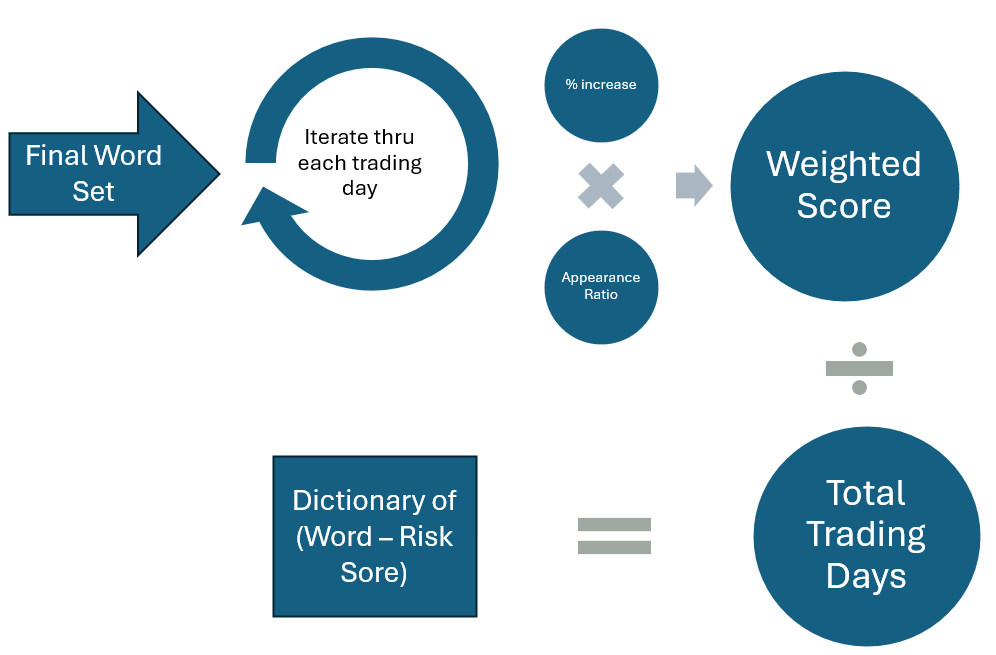
\includegraphics[width=0.5\textwidth]{Risk Score Calculation.png}
        \caption{Alternative Risk Score Calculation.}
        \label{fig:risk score calculation}
    \end{figure}        
\end{enumerate}

We ran two kinds of prediction: regression and classification and we use multiple metrics to measure and compare model performance:
\begin{enumerate}
    \item \textbf{Regression:} Measure - mean absolute error and R-square.
    \item \textbf{Classification:} Measure - Precision, Recall and F1 score.
\end{enumerate}
We chose these classification measures because the positive identification of the stock price drop is important to us. 

Because we have done comparison of different regression methods in other part of this report, we are only using XGboost to simplify the comparison process. 

\subsection{Regression Analysis and Comparison:}
We started our initial analysis with multiple individual features, most of which provide a negative or low R-square value. Risk Score feature is the only one that shows a good R-square result. We then try adding other features to see if the performance can improve. We found a combination of Vix and Risk Score significantly improves R-square value. This is clearly illustrated in the Vix and Risk Score Interaction table.  This improved performance could be due to the non-linear effects that emerge when both are present. In our case, Vix adds context to Risk Score. Keep in mind, our XGboost method automatically captures interaction and does not require additional interaction feature. 

Similarly to the previous risk score method, we also noticed the impact of the count of articles. As the total number of articles increased, the performance of our model increased dramatically. As we observed on the Vix and Risk Score fig \ref{fig:vix and risk score}, with both variables features, MAE decreased from 2.04 to 0.85 as we increase the number of article. In addition, the R-square value increased from 0.08 to 0.61. This also makes sense, as more data generally means:
\begin{enumerate}
    \item \text Less noise.
    \item \text Variance is more stable.
    \item \text Model can detect patterns more reliably.
    \item \text Reduction in overfitting effects. A small sample might not capture the true variability.
\end{enumerate}

\begin{figure}[ht]
    \centering
    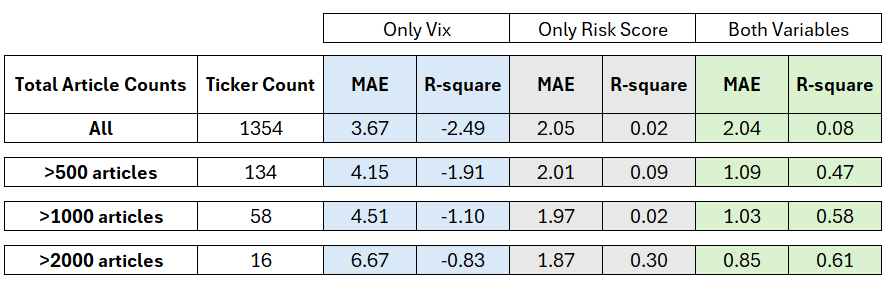
\includegraphics[width=0.5\textwidth]{vix and risk score interaction table.png}
    \caption{Vix and Risk Score Interaction.}
    \label{fig:vix and risk score}
\end{figure}

\subsection{Classification Categorization:}
While regression prediction is important for our analysis, classification/categorization is more meaningful for investors. Because investors can trigger actions easier based on different scenario/categorization. For our analysis, we break the daily percentage change into 6 categories/groups/scenarios per table \ref{tab:Daily Stock Percetage change Categories.}.

\begin{table}[h!]
\centering
\normalsize
\begin{tabular}{|l|c|}
\hline
\textbf{Group} & \textbf{Label} \\
\hline
1 & Big Gain \\
2 & Moderate Gain \\
3 & Small Gain \\
4 & Small Drop \\
5 & Moderate Drop \\
6 & Big Drop \\

\hline
\end{tabular}
\caption{Daily Stock Percentage Change Group.}
\label{tab:Daily Stock Percetage change Categories.}
\end{table}

It is common for different stocks to have different volatility. For instance, it is not typical for Apple stock to move up and down 5 percentage within a day. However, that is not uncommon for highly volatile stocks such as SMCI. This is perfectly illustrated in fig \ref{fig:ave abs stock change}.  where it lists the average daily stock price change percentage (in absolute value) So the definition of big gain or big drop will really depend on stock volatility.    

\begin{figure}[ht]
    \centering
    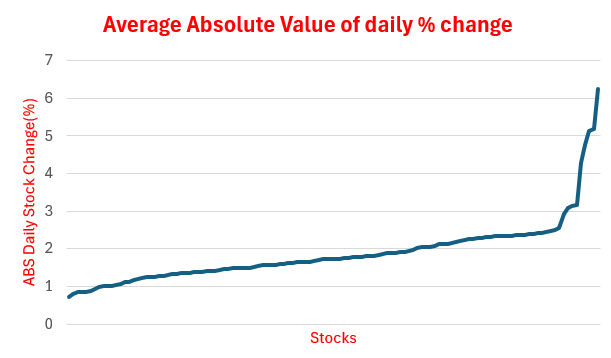
\includegraphics[width=0.5\textwidth]{Average ABS value of daily stock change.png}
    \caption{Average Absolute Value of Daily Stock Price Change.}
    \label{fig:ave abs stock change}
\end{figure}
To reflect this volatility, we introduced 4 different sets of groupings based on their average daily stock price change. The exact breakdown is shown in fig \ref{fig:daily stock price sets}.

\begin{figure}[ht]
    \centering
    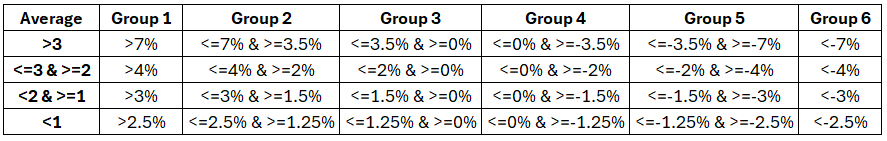
\includegraphics[width=0.5\textwidth]{daily stock price change sets.png}
    \caption{Daily Stock Price Change Grouping Sets.}
    \label{fig:daily stock price sets}
\end{figure}

One of our primary goals is to warn investor about a potential stock price drop. In our modeling, we combine groups 5 and 6 (Moderate Drop and Big Drop) into one group and rest to another group. We then see how accurate we are at predicting correctly groups 5 and 6. There are many measures we could use to see our classification accuracy. If false positive is more costly we should use precision.  On the other hand, F1 score is a balanced metric between the two.  

\begin{figure}[ht]
    \centering
    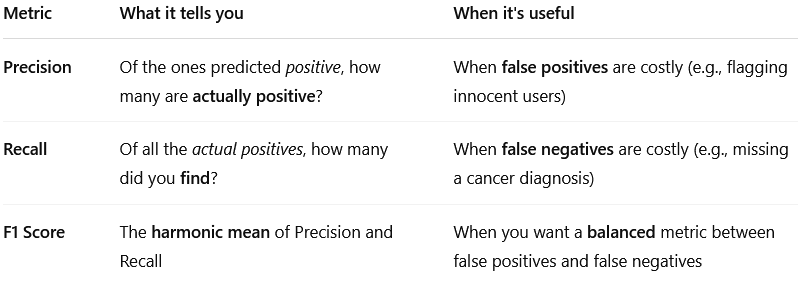
\includegraphics[width=0.5\textwidth]{classification metric comparison.png}
    \caption{Classification Metric Comparison.}
    \label{fig:classificait metric comparison}
\end{figure}

Our classification result fig \ref{fig:classificait result}, shows similar observation vs article count. Just as we saw in regression analysis, higher article count corresponds to higher performance. This is caused by same reasons stated previously.

\begin{figure}[ht]
    \centering
    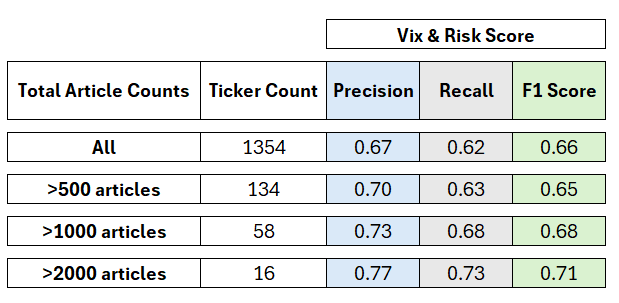
\includegraphics[width=0.5\textwidth]{classification result.png}
    \caption{Classification Result.}
    \label{fig:classificait result}
\end{figure}

\subsection{Technical Analysis:}
NLP/Machine Learning is our primary focus for stock price prediction. There are two other major approaches:
\begin{enumerate}
    \item \textbf{Technical Analysis:} Uses historical price and volume data to identify trends, patterns, and signals. In our case, we use:
        \begin{enumerate}
            \item \ Bollinger Band.
            \item \ Relative Strength Index (RSI).
            \item \ Stochastic Oscillator. 
        \end{enumerate}
    \item \textbf{Fundamental Analysis:} Focuses on company financial, industry health, and macroeconomic factors (e.g. P/E ratio, revenue growth, earnings reports). 
\end{enumerate}

We want to incorporate one additional method and see if it will improve our model performance. Fundamental analysis will require very comprehensive financial information of each company and it will be difficult to obtain and incorporate into our model. Technical analysis, on the other hand, is relatively easy as we already have price data. We choose Bollinger Band, RSI and Stochastic Oscillator as those are relatively easy to calculate and are based on information we already have. Unfortunately, we did not see a performance improvement by adding these information. In contrast, we actually saw a performance degradation fig \ref{fig:result TA} . We believe this degradation is due to additional noise introduced by 6 more TA features. Reinforcement learning (RL) might be a better method for the following reasons:

\begin{enumerate}
    \item \ More strategic instead of static. 
    \item \ Has temporal awareness. RL models sequence or long term dependencies.
\end{enumerate}

\begin{figure}[ht]
    \centering
    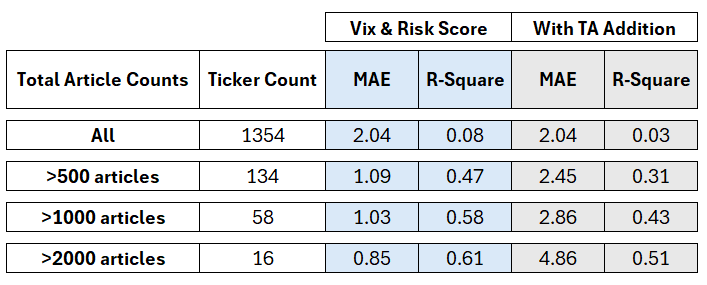
\includegraphics[width=0.5\textwidth]{result with TA addtion.png}
    \caption{Model Performance Comparison with Addition of Technical Analysis.}
    \label{fig:result TA}
\end{figure}

Due to time constraints and the complexity of the RL method, we did not incorporate RL into our analysis. That could be something we recommend as a future action. 

\subsection{Summary}
\begin{enumerate}
    \item \textbf{VIX and Risk Score interaction improve model performance:} Each Vix is a weak feature individually and Risk Score performs much better with Vix added.

    \item \textbf{Article count has big impact on performance:} Higher article count leads to higher performance for both regression and classification analysis.  

    \item This comparison reaffirms our earlier conclusion that token-based sentiment metrics, rather than traditional technical indicators, offer greater predictive power in this context.

\end{enumerate}

%%%%%%%%%%%%%%%%%%%%%%%%%%%%%%%%%%%%%%%%%%%%%%%%%%%%%%%%%%%%%%%%%%%%%%
%% Topic Modeling Approach
%%%%%%%%%%%%%%%%%%%%%%%%%%%%%%%%%%%%%%%%%%%%%%%%%%%%%%%%%%%%%%%%%%%%%%

\section{Topic Modeling Approach}
Our topic modeling approach leverages \textbf{BERTopic} to extract latent themes from financial news articles. By converting unstructured text into topic-based features, we can capture underlying market sentiments and risk signals that improve stock price movement predictions.

\subsection{Methodology and Model Parameters}
We follow a multi-step pipeline:
\begin{enumerate}
    \item \textbf{Text Preprocessing:} Articles are cleaned, tokenized, and lemmatized. Stopwords and non-informative tokens are removed.
    \item \textbf{Embedding Generation:} We compute sentence embeddings using the \texttt{SentenceTransformer} model \texttt{"paraphrase-MiniLM-L3-v2"}.
    \item \textbf{Dimensionality Reduction:} UMAP is applied with parameters: \texttt{n\_neighbors = 5}, \texttt{min\_dist = 0.5}, and \texttt{n\_components = 5}.
    \item \textbf{Topic Extraction:} BERTopic is then used to cluster the embeddings into topics. We experimented with different numbers of topics (e.g., $K=5$, 10, 15) and found that $K=10$ offers the best balance between topic granularity and coherence (average coherence $\approx 0.42$).
\end{enumerate}

\subsection{Feature Engineering}
Once each article is assigned a distribution over topics, we aggregate topic information at the ticker-day level by computing several features:
\begin{itemize}
    \item \textbf{\texttt{topic\_avg\_movement}:} The historical average return for each topic.
    \item \textbf{\texttt{topic\_sensitivity}:} The standard deviation of returns associated with each topic.
    \item \textbf{\texttt{sentiment\_impact}:} Derived from FinBERT analysis as the difference between positive and negative sentiment scores.
    \item \textbf{\texttt{market\_volatility}:} A 30-day rolling standard deviation of the price change percentage.
\end{itemize}

This process helps identify clusters of event-driven themes—such as legal, earnings, or M\&A news—that have been shown to carry predictive value in prior event-based financial modeling research~\cite{hu2018}.

These engineered features serve as inputs to our per-ticker predictive models.

\subsection{Per-Ticker Modeling and Quantitative Results}
To evaluate the predictive power of topic-based features, we trained separate XGBoost regressors for each ticker with:
\begin{itemize}
    \item \textbf{Target:} Daily price change percentage.
    \item \textbf{Metrics:} Mean Absolute Error (MAE) and R\textsuperscript{2} score.
    \item \textbf{Feature Correlations:} Pearson correlations between each feature and the price change target. For example, correlations (in absolute value) range from about 0.05 to 0.62, indicating that the features are moderately predictive.
\end{itemize}

Table~\ref{tab:topic_model_results} (values provided here are illustrative) summarizes these metrics:

\begin{table}[h!]
\centering
\small
\begin{tabular}{|l|c|}
\hline
\textbf{Feature} & \textbf{Correlation (r)} \\
\hline
topic\_avg\_movement & 0.25 \\
topic\_sensitivity   & 0.09 \\
sentiment\_impact    & 0.07 \\
market\_volatility   & 0.08 \\
risk\_score\_topic   & 0.11 \\
\hline
\end{tabular}
\caption{Summary of feature correlations with the price change target.}
\label{tab:topic_model_results}
\end{table}

\subsection{Impact of Article Volume on Model Performance}
We further investigated how the number of articles per ticker affects model performance:
\begin{itemize}
    \item Tickers with fewer than 100 articles generally exhibit poor performance.
    \item Tickers with more than 250 articles show a significant improvement in R\textsuperscript{2} scores (e.g., a median R\textsuperscript{2} around 0.57).
\end{itemize}

Figure~\ref{fig:article-volume-reg} displays a scatter plot (with the number of articles on a logarithmic scale) versus R\textsuperscript{2} scores, overlaid with a regression line. In Figure~\ref{fig:article-volume-lowess}, a LOWESS smoothed curve further highlights the positive trend between article volume and model performance.

\begin{figure}[h!]
    \centering
    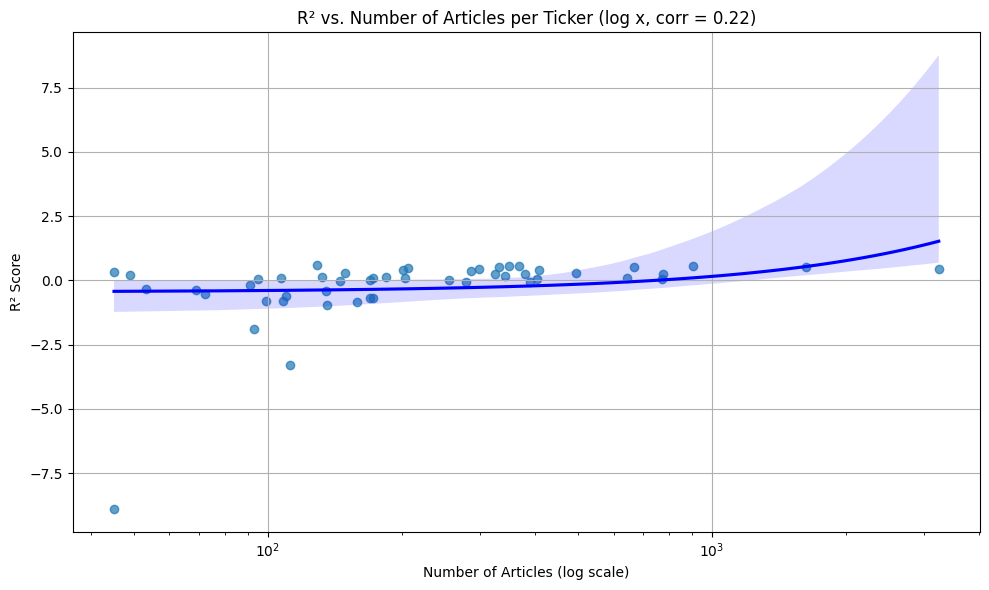
\includegraphics[width=0.5\textwidth]{log_scale_article_mod_performance.png}
    \caption{Scatter plot of number of articles per ticker vs. R\textsuperscript{2} score with a regression line.}
    \label{fig:article-volume-reg}
\end{figure}

\begin{figure}[h!]
    \centering
    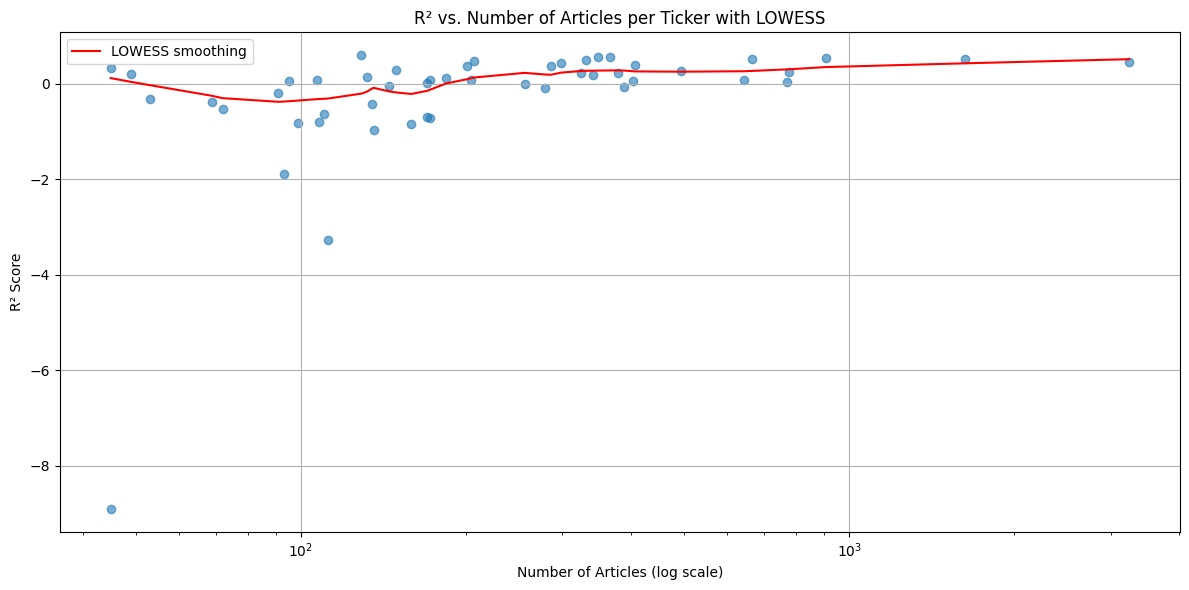
\includegraphics[width=0.5\textwidth]{lowess_smoothing.png}
    \caption{LOWESS smoothed trend of ticker article volume (log scale) vs. R\textsuperscript{2} score.}
    \label{fig:article-volume-lowess}
\end{figure}

\subsection{Summary}
This topic modeling framework not only captures latent themes in financial news using BERTopic but also translates them into meaningful features that enhance per-ticker stock price movement prediction. The integration of topic-based features with sentiment analysis and article volume metrics has led to improved predictive performance—especially for tickers with a higher volume of news. This method showed particular strength for tickers with a large volume of articles, suggesting that topic-based features are especially valuable in high-coverage environments.

\section{Short-Term vs. Long-Term Opportunities}

This project has laid foundational groundwork on modeling stock volatility using sentiment and token-based risk features. Should this work be extended, there are several promising approaches to deepen the analysis and enhance predictive performance.

Not all enhancements have equal feasibility or time requirements. We identify a few that are viable in the short term versus others that require more R\&D investment:

\begin{itemize} 
    \item \textbf{Short-Term:} Segmentation, adaptive ensembles, multi-feature fine-tuning.
    \item \textbf{Long-Term:} Reinforcement learning, mixture-of-experts, and hierarchical multitask models.
\end{itemize}

\subsection{Segmentation or Clustering}

\textbf{Concept:} 
Group stocks based on similar characteristics such as market capitalization, article volume, or model performance metrics (e.g., MAE and $R^2$), aiming for more homogeneous data clusters.

\textbf{Implementation Ideas:}

\begin{itemize}
    \item \textbf{Unsupervised Clustering:} Apply algorithms like k-means, hierarchical clustering, or DBSCAN on relevant features to discover inherent groupings, e.g., high-cap versus low-cap stocks.
    \item \textbf{Domain-Based Segmentation:} Explicitly segment stocks based on predefined criteria (small, mid, large-cap) and create tailored predictive models for each segment.
\end{itemize}

\textbf{Pros and Cons:}
\begin{itemize}
    \item \textit{Pros:} Specialized models for distinct groups, better handling of data sparsity.
    \item \textit{Cons:} Potential complexity in cluster boundary definitions and feature normalization.
\end{itemize}

\subsection{Mixture-of-Experts Models}

\textbf{Concept:} 
Develop multiple specialized predictive models ("experts"), each suited to particular stock subsets or market conditions. A gating model dynamically assigns weights to each expert’s prediction.

\textbf{Implementation Ideas:}

\begin{itemize}
    \item \textbf{Expert Networks:} Train neural networks on distinct subsets or conditions.
    \item \textbf{Gating Mechanism:} Utilize a secondary model to dynamically determine expert weighting based on input features.
    \item \textbf{Dynamic Adaptation:} Continuously update the gating model to respond to evolving market dynamics.
\end{itemize}

\textbf{Pros and Cons:}
\begin{itemize}
    \item \textit{Pros:} Flexibility, dynamic responsiveness to market conditions.
    \item \textit{Cons:} Increased complexity, risk of overfitting, higher computational demands.
\end{itemize}

\subsection{Multi-Task or Hierarchical Modeling}

\textbf{Concept:} 
View each stock prediction as a distinct but related task, leveraging shared information to inform predictions across tasks.

\textbf{Implementation Ideas:}

\begin{itemize}
    \item \textbf{Multi-Task Neural Networks:} Employ shared layers for general trends and task-specific layers for individual stock nuances.
    \item \textbf{Hierarchical Bayesian Models:} Assume parameters for each stock come from a common distribution, sharing strength between data-rich and sparse stocks.
\end{itemize}

\textbf{Pros and Cons:}
\begin{itemize}
    \item \textit{Pros:} Better predictions for stocks with limited data, captures both shared and individual patterns.
    \item \textit{Cons:} Complex model structures, careful balancing required to retain stock-specific details.
\end{itemize}

\subsection{Adaptive Weighting in Ensemble Methods}

\textbf{Concept:} 
Employ ensembles of models, adaptively weighting contributions based on historical performance under specific conditions.

\textbf{Implementation Ideas:}

\begin{itemize}
    \item \textbf{Stacking and Blending:} Combine predictions from multiple models using a meta-model informed by past accuracy.
    \item \textbf{Performance-Based Weighting:} Dynamically adjust ensemble weights based on recent prediction accuracy.
    \item \textbf{Adaptive Algorithms:} Use boosting methods to iteratively focus on correcting previous model errors.
\end{itemize}

\textbf{Pros and Cons:}
\begin{itemize}
    \item \textit{Pros:} Enhanced overall predictive accuracy, adaptability.
    \item \textit{Cons:} Increased complexity, potential for overfitting.
\end{itemize}

\subsection{Incorporate Reinforcement Learning}

\textbf{Concept:} 
Enhance technical Analysis and NLP based analysis by using Reinforcement Learning to training an agent to make decisions by interacting with an environment to maximize rewards over time.

\textbf{Technical Analysis Implementation Steps:}

\begin{itemize}
    \item \textbf{Define the Environment:} Use gym-anytrading or FinRL for financial RL environment. Define states, action space and rewards.
    \item \textbf{Choose an RL Algorithm:} Choose either Deep Q-Learning (DQN), PPO, A2C or DDPG.
    \item \textbf{Build the Agent:} Use neural network architecture that maps state → action values or probabilities). Train using the chosen RL algorithm.
    \item \textbf{Train the Agent:} Choose neural network architecture that maps state → action values or probabilities. Use backpropagation and experience replay (for DQN) or advantage estimations (for PPO). 
    \item \textbf{Back test and Evaluate:} Test the trained agent on unseen data. Compare to benchmarks.
\end{itemize}

\textbf{NLP Based Analysis:}
\begin{itemize}
    \item \textbf{Extract Features with NLP:} Apply NLP models to get article embeddings or sentiment scores.
    \item \textbf{Create State Representations:} Combine NLP features with market indicators. 
    \item \textbf{Define the RL Trading Environment:} Define state, actin space, reward and episode.
    \item \textbf{Choose and Train the RL Agent:} Select RL algorithm, similar algorithms listed for technical analysis. Train the agent by simulating trading over historical news and price data.
    \item \textbf{Back test and Evaluate:} Compare to baseline strategies. Evaluate metrics. 
\end{itemize}



\subsection{Final Thoughts}

Selecting an optimal approach—or a combination thereof—depends on practical constraints, data availability, and computational resources. Often, hybrid strategies, such as segmenting data and using mixture-of-experts or multi-task frameworks enhanced by additional data streams, provide the most robust outcomes. Future work could involve iterative prototyping, rigorous validation against historical data, and careful evaluation of practical constraints.

\section{Workload Distribution}
\begin{itemize}
    \item \textbf{Luis Tupac:} In charge of database creation and maintenance, data pipelines, and data transformation; FinBERT sentiment classification on financial reports, headline news, and new testing data. Worked on VIX Time Series Modeling and Thematic Clustering approaches. 
    \item \textbf{Brian Adams:} Exploratory data analysis, experimenting with the calculation of risk scores, and exploring different modeling approaches (topic modeling, token score with sentiment).
    \item \textbf{Hilung Huang:} Overall project approach, initial modeling, alternative risk score method, Named Entity Recognition enhancement, technical analysis addition, and coordination of tasks.
\end{itemize}

\section{Conclusion}

This project has extensively demonstrated the potential of NLP-driven approaches to predict market volatility through detailed analysis of financial sentiment indicators. We systematically explored and compared various modeling strategies, including token-level sentiment analytics, volatility forecasting using VIX, topic modeling, and multi-feature ensembles. Our results clearly indicate that models integrating comprehensive token-based risk scores significantly outperform simpler sentiment-only models, validating our initial hypotheses regarding the importance of nuanced textual insights.

We also found that predictive accuracy greatly benefits from adequate data volume and carefully engineered and aggregated features. Our experiments underscore the importance of balancing model complexity with robustness, highlighting that streamlined, thoughtfully constructed features often provide the most stable predictions.

Future efforts extending this work should focus on advanced hybrid approaches, such as segmentation-based clustering, hierarchical multitask modeling, dynamic ensemble methods, and reinforcement learning as outlined in our recommended next steps. Ultimately, by continuing to refine these methods and rigorously validating them against diverse market conditions, the proposed sentiment-based Risk Scores can evolve into powerful, actionable tools for investors aiming to anticipate and respond effectively to market inflection points.


\bibliographystyle{plain}
\bibliography{references}
% \begin{thebibliography}{9}

% \bibitem{bollinger}
% ChartSchool. \textit{Bollinger Bands}. Retrieved from \url{https://school.stockcharts.com/doku.php?id=technical_indicators:bollinger_bands} (Accessed: April 4, 2025)

% \bibitem{rsi}
% ChartSchool. \textit{Relative Strength Index (RSI)}. Retrieved from \url{https://school.stockcharts.com/doku.php?id=technical_indicators:relative_strength_index_rsi} (Accessed: April 4, 2025)

% \bibitem{stochastic}
% ChartSchool. \textit{Stochastic Oscillator}. Retrieved from \url{https://school.stockcharts.com/doku.php?id=technical_indicators:stochastic_oscillator_fast_slow_and_full} (Accessed: April 4, 2025)

% \end{thebibliography}

\end{document}